\documentclass[aspectratio=169]{beamer}
\usetheme{Madrid}

\usepackage{graphicx}
\usepackage[utf8]{inputenc}
\usepackage{hyperref}
\usepackage{listings}
\usepackage{subcaption}
\usepackage{tikz}
\usetikzlibrary{shapes, arrows, positioning}

%\setbeamertemplate{footline}[frame number]

\begin{document}

\title{Neural Networks and Deep Learning}  
\subtitle{Transformers} 
\author[J.I. Vasquez]{\textbf{Juan Irving Vásquez} \\jivg.org}
\date{\today \copyright}
\institute[jivg.org]{Centro de Innovación y Desarrollo Tecnológico en Cómputo \\ Instituto Politécnico Nacional}
\titlegraphic{
\includegraphics[height=1.2cm]{ipn-cidetec.png}\hspace{0.1cm}
\includegraphics[height=1.2cm]{escudoESCOM}}
\frame{\titlepage} 

\frame{
	\frametitle{Contents}
	\tableofcontents
}

\AtBeginSection[] { \begin{frame} \frametitle{Roadmap} \tableofcontents[currentsection] \end{frame} }

\section{Preliminaries}



% --- Diapositiva 1: Problemas de Información ---
\begin{frame}{Issues with RNN-based Encoder-Decoder (1/2)}
	\begin{columns}[c] % [c] alinea verticalmente al centro
		% Columna de Texto
		\begin{column}{0.6\textwidth}
			The Seq2Seq architecture laid the groundwork. \\ Limitations:
			
			\begin{enumerate}
				\item \textbf{Information bottleneck:}
				\begin{itemize}
					\item Compressing the entire source sentence into a single context vector leads to loss of information, especially for long sequences.
				\end{itemize}
				
				\item \textbf{Long-distance dependencies:}
				\begin{itemize}
					\item Complex sentence structures make it difficult for a single vector to capture relationships between distant words.
				\end{itemize}
			\end{enumerate}
		\end{column}
	
		\pause
		
		% Columna de Imagen
		\begin{column}{0.4\textwidth}
			\centering
			%Reemplaza la siguiente línea con
			
\includegraphics[width=0.75\textwidth]{51457rnnmemory.png}
			%\rule{\textwidth}{3cm} % Placeholder para imagen
			%\tiny{\textit{Visual representation of the information bottleneck.}}
		\end{column}
	\end{columns}
\end{frame}

% --- Diapositiva 2: Problemas Computacionales ---
\begin{frame}{Issues with RNN-based Encoder-Decoder (2/2)}
	\begin{columns}[c]
		% Columna de Texto
		\begin{column}{0.6\textwidth}
			Additionally, the recurrent nature introduces training and hardware challenges:
			
			\begin{enumerate}
				\setcounter{enumi}{2} % Reinicia el contador en 3
				\item \textbf{Optimization issues:}
				\begin{itemize}
					\item RNNs are prone to vanishing and exploding gradients, making training unstable.
				\end{itemize}
				\pause
				\item \textbf{Computational inefficiency:}
				\begin{itemize}
					\item The recurrence (dependence on $t-1$) makes parallelization impossible, leading to slower training times.
				\end{itemize}
			\end{enumerate}
			
			\vspace{0.4cm}
			\small\textit{These limitations paved the way for the Attention Mechanism and Transformers.}
		\end{column}
		
		% Columna de Imagen
		\begin{column}{0.4\textwidth}
			\centering
			% Reemplaza la siguiente línea con 
			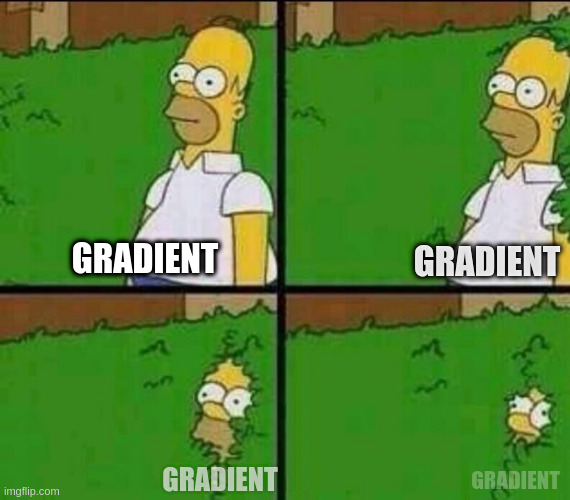
\includegraphics[width=0.9\textwidth]{FGAA_iyXIAcdVI5.jpg}
			%\rule{\textwidth}{3cm} % Placeholder para imagen
			%\tiny{\textit{Sequential processing inhibits parallelization.}}
		\end{column}
	\end{columns}
\end{frame}





\section{Motivation}


\frame{
	\frametitle{The A.I. revolution}
	\begin{columns}[c] % El parámetro [c] alinea el contenido verticalmente al centro
		
		% --- Columna Izquierda (Texto) ---
		\begin{column}{0.5\textwidth}
			\begin{itemize}
				\item ChatGPT became publicly available in November 30 2022\footnote{Gemini, Consulted May 26.}
				\item It reached 100 million users in just two months.
				\item 550 M in 2025.
			\end{itemize}
		\end{column}
		
		% --- Columna Derecha (Imagen) ---
		\begin{column}{0.5\textwidth}
			\begin{figure}
				\centering
				% Ajusté el ancho a \linewidth para que se adapte al tamaño de su columna
				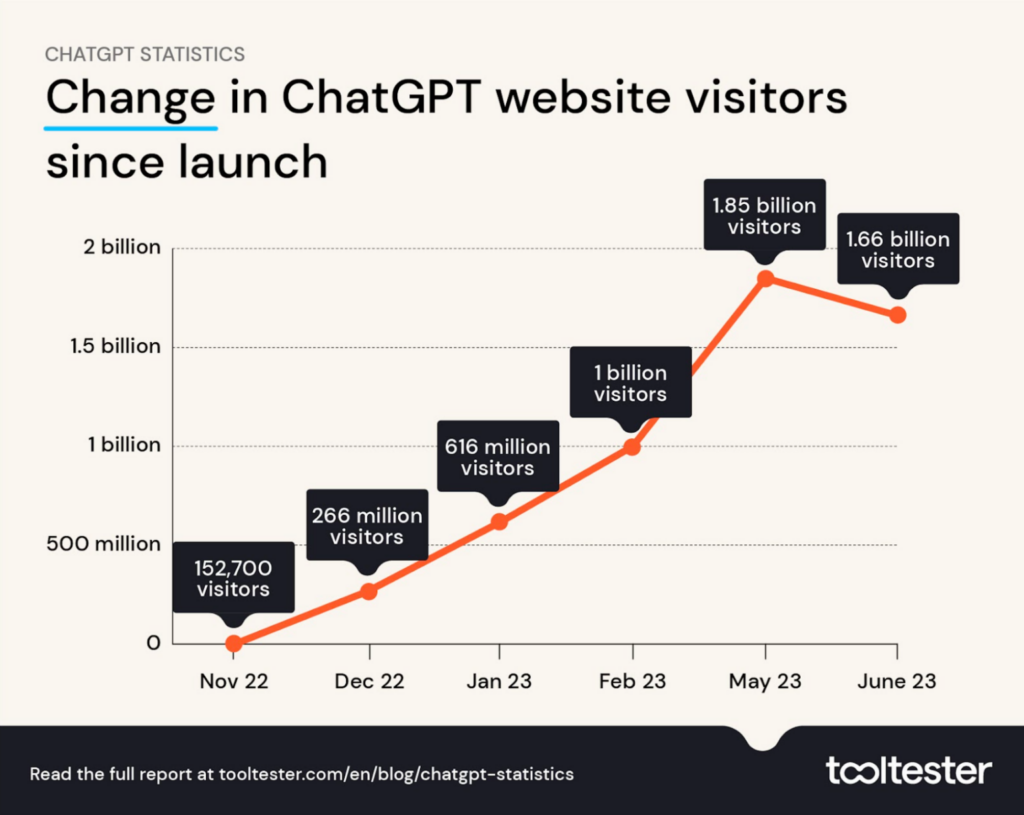
\includegraphics[width=\linewidth]{chatgpt-user} 
				\caption{}
				\label{fig:chatgpt-user}
			\end{figure}
		\end{column}
	\end{columns}
}


\frame{
	\frametitle{Advances in science}
	\begin{columns}[c] % El parámetro [c] alinea el contenido verticalmente al centro
		
		% --- Columna Izquierda (Texto) ---
		\begin{column}{0.5\textwidth}
			\begin{itemize}
				\item ChatGPT became publicly available in November 30 2022\footnote{Gemini, Consulted May 26.}
				\item It reached 100 million users in just two months.
				\item 550 M in 2025.
			\end{itemize}
		\end{column}
		
		% --- Columna Derecha (Imagen) ---
		\begin{column}{0.5\textwidth}
			\begin{figure}
				\centering
				% Ajusté el ancho a \linewidth para que se adapte al tamaño de su columna
				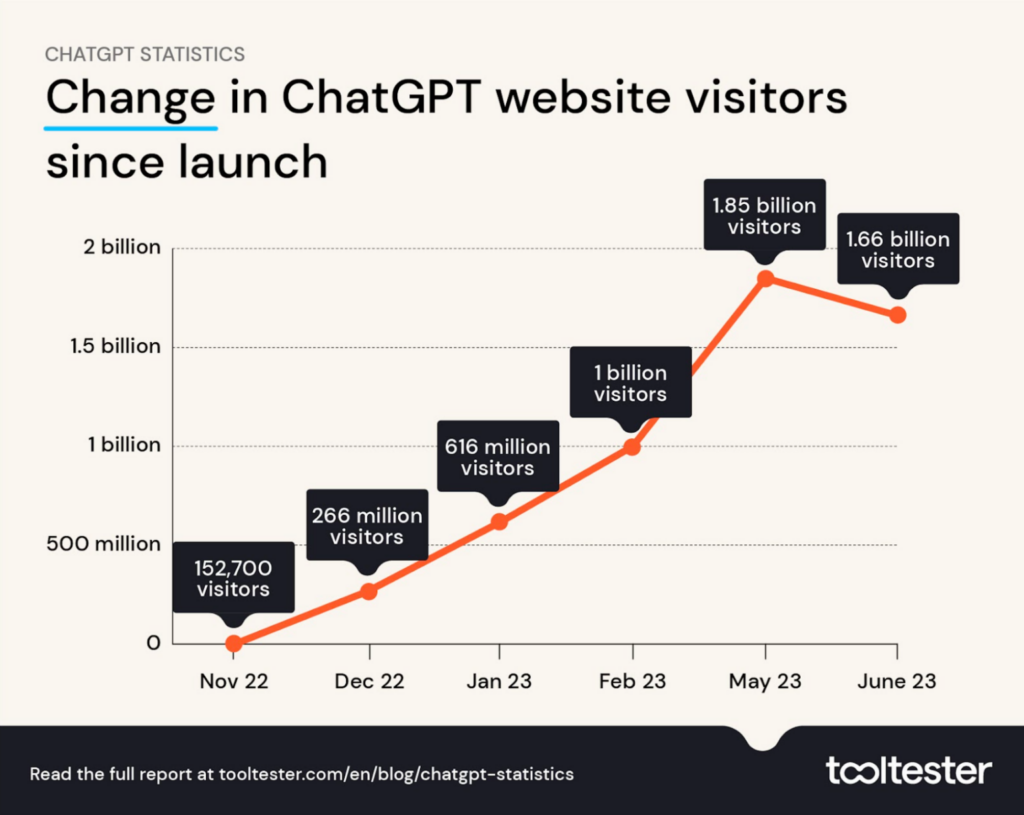
\includegraphics[width=\linewidth]{chatgpt-user} 
				\caption{}
				\label{fig:chatgpt-user}
			\end{figure}
		\end{column}
	\end{columns}
}


\section{The Transformer arrise}


\begin{frame}
	\centering
	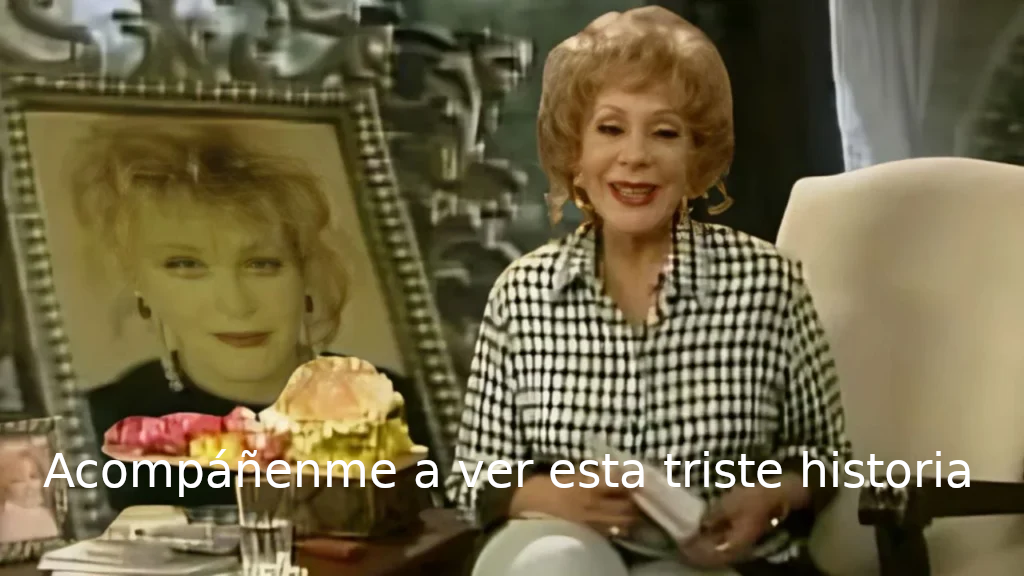
\includegraphics[width=0.8\linewidth]{silvia}
\end{frame}


\begin{frame}
	\begin{figure}
		\centering
		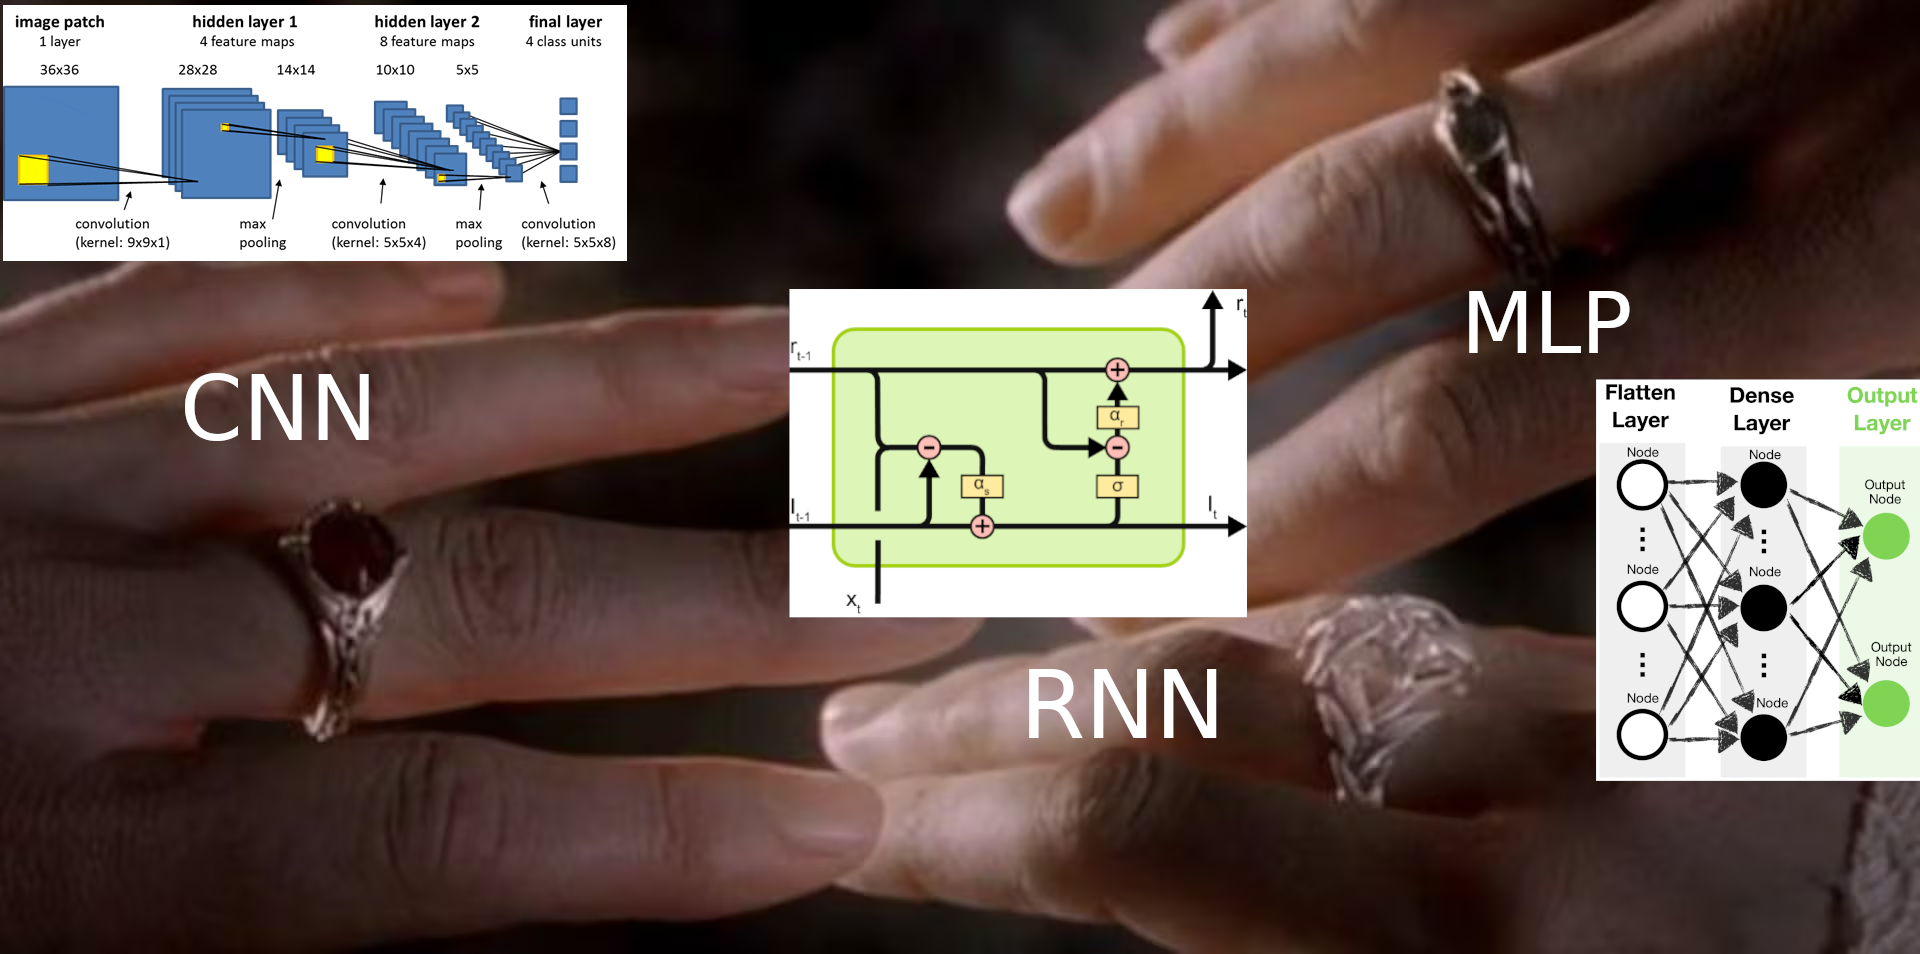
\includegraphics[width=0.8\linewidth]{anillos_redes}\caption{En la segunda era del silicio, los grandes científicos de datos forjaron las \textbf{redes del poder}.}	
	\end{figure}
\end{frame}


\begin{frame}
	\begin{figure}
		\centering
		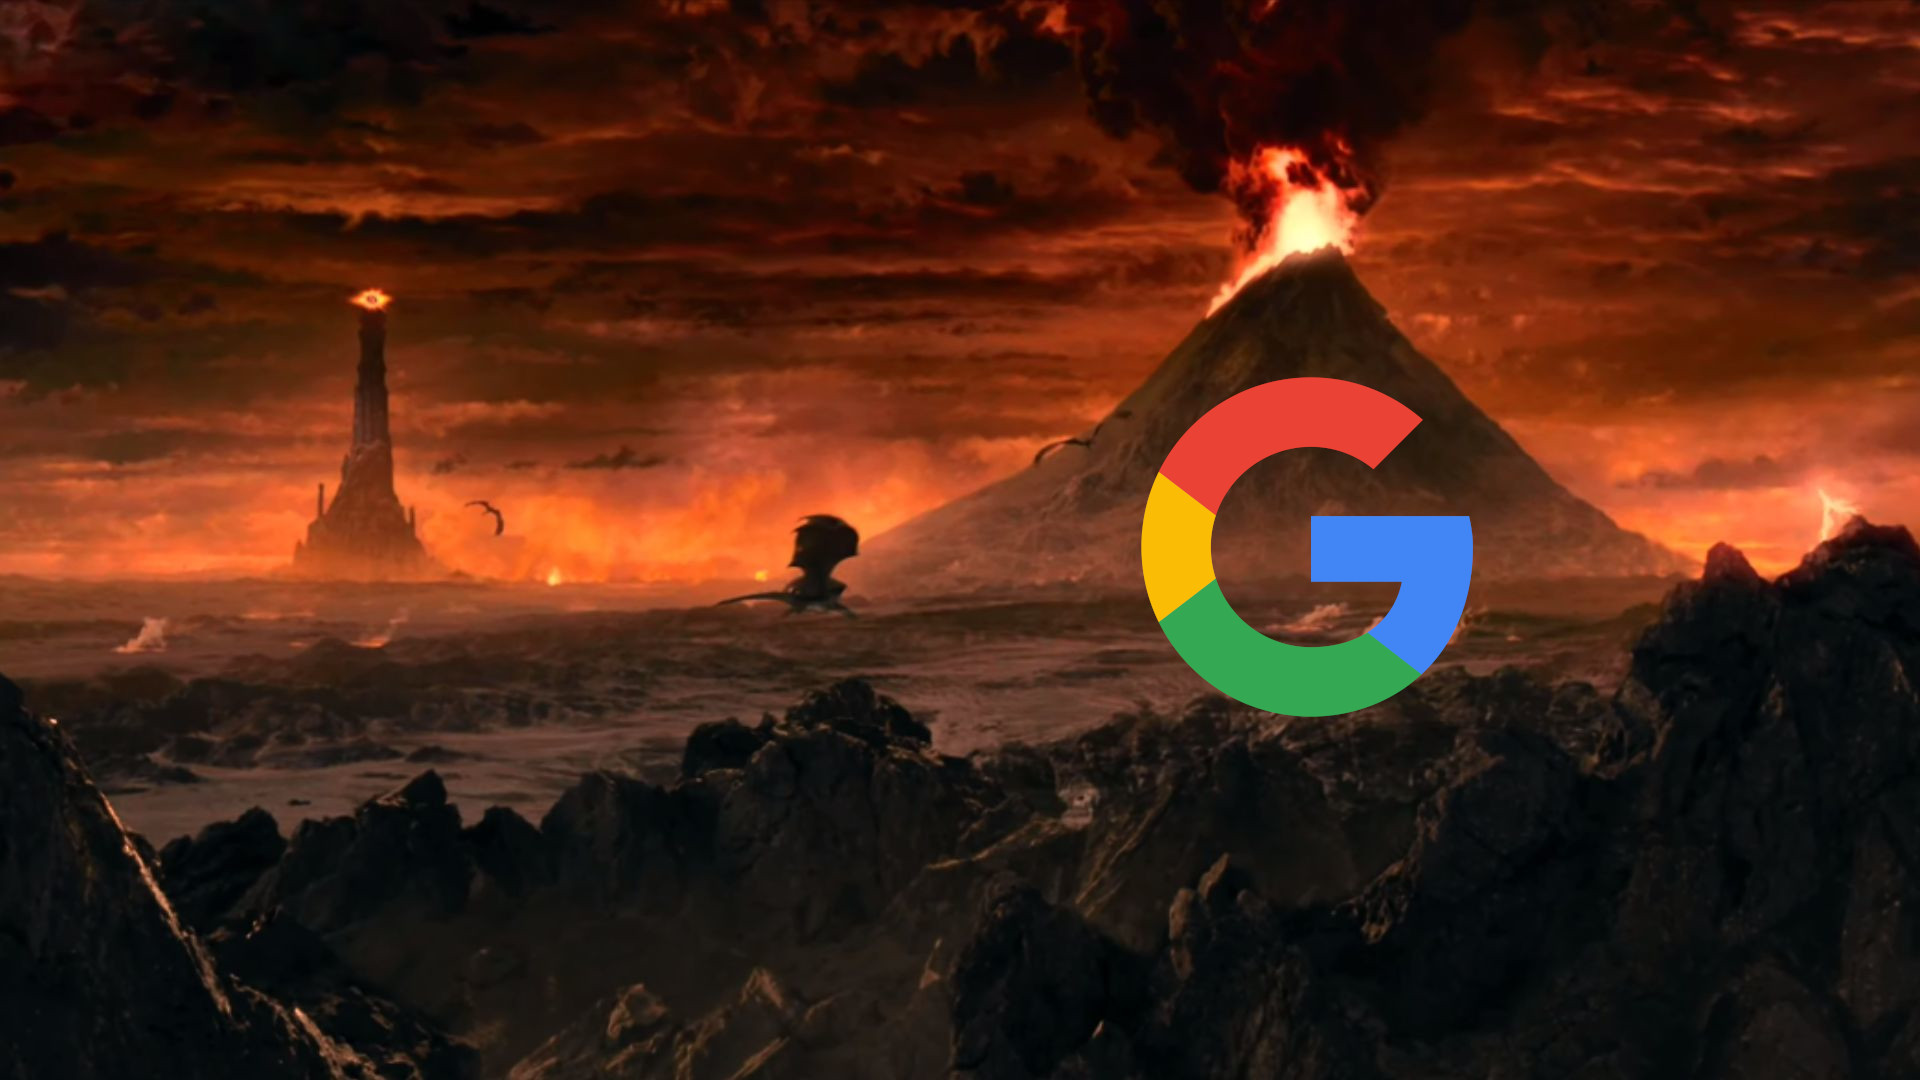
\includegraphics[width=0.8\linewidth]{mordor}	
		\caption{Pero en los laboratorios de Mordoogle un cónclave de ingenieros trabajaba en secreto.}
	\end{figure}
\end{frame}


\begin{frame}
\begin{figure}
	\centering
	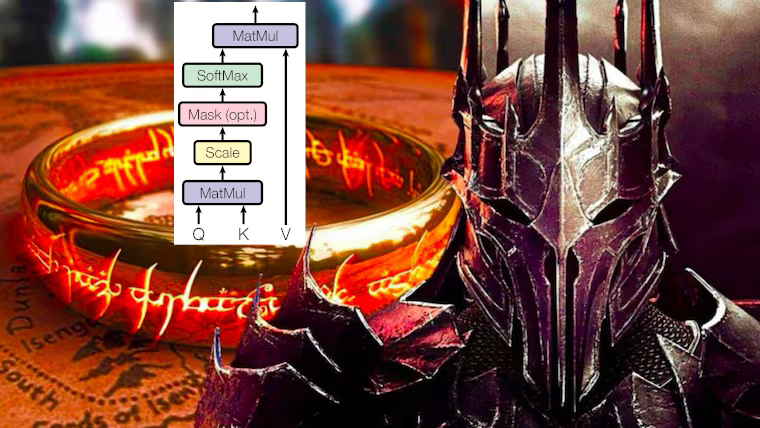
\includegraphics[width=0.8\linewidth]{ring_att}
	\caption{Jakob Uszkoreit y sus aliados forjaron un mecanismo capaz de modelar relaciones entre cualquier tipo de dato}
\end{figure}
\end{frame}


\frame{
\frametitle{The paper that made the revolution}
%\begin{figure}
	\centering
	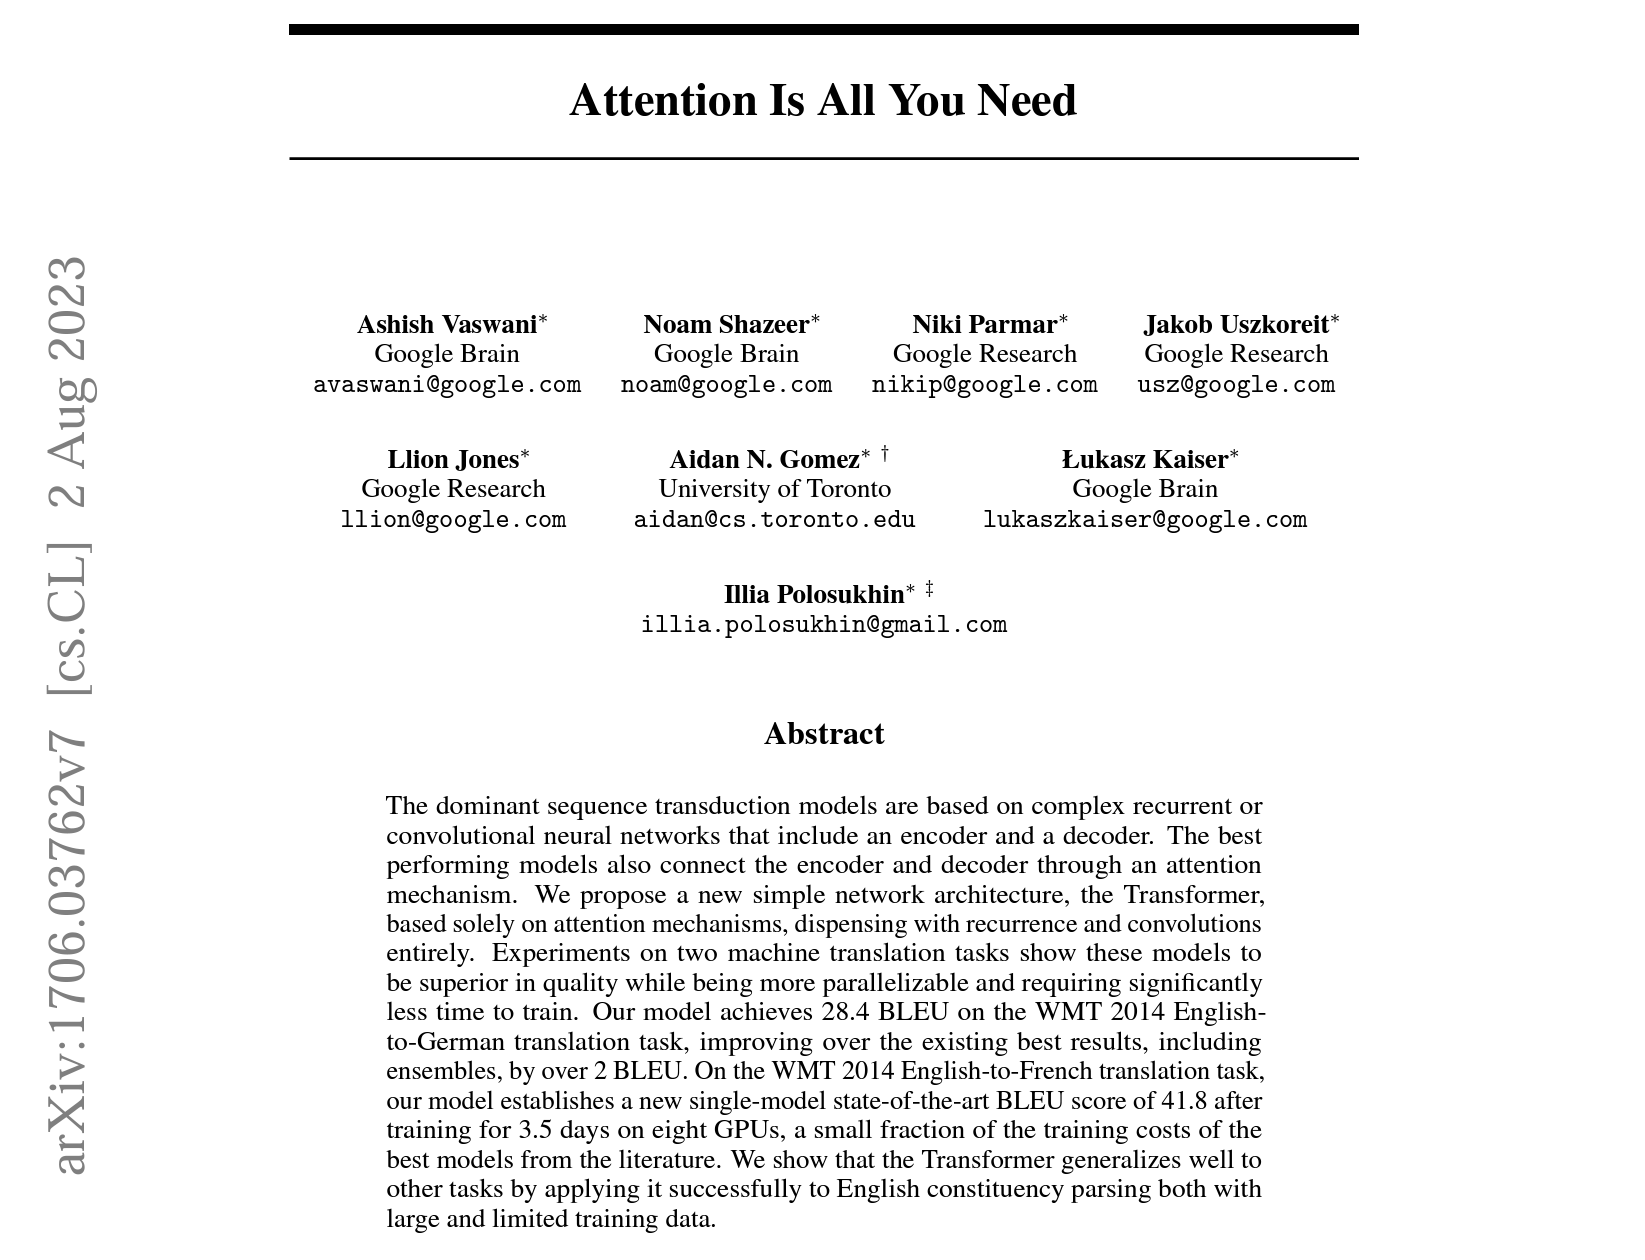
\includegraphics[width=0.6\linewidth]{aisyn}
%	\pause
%	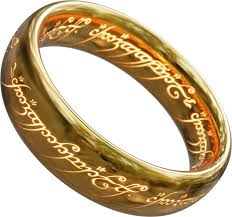
\includegraphics[width=0.2\linewidth]{ring.jpeg}
%	\caption{}
%	\label{fig:aisyn}
%\end{figure}
}


\begin{frame}
	\frametitle{8 Google Employees Invented Modern AI\footnote{\scriptsize Steven Levy, "8 Google Employees Invented Modern AI. Here’s the Inside Story," Wired, 20 de marzo de 2024}}
\begin{figure}
	\begin{subfigure}{0.15\textwidth}
	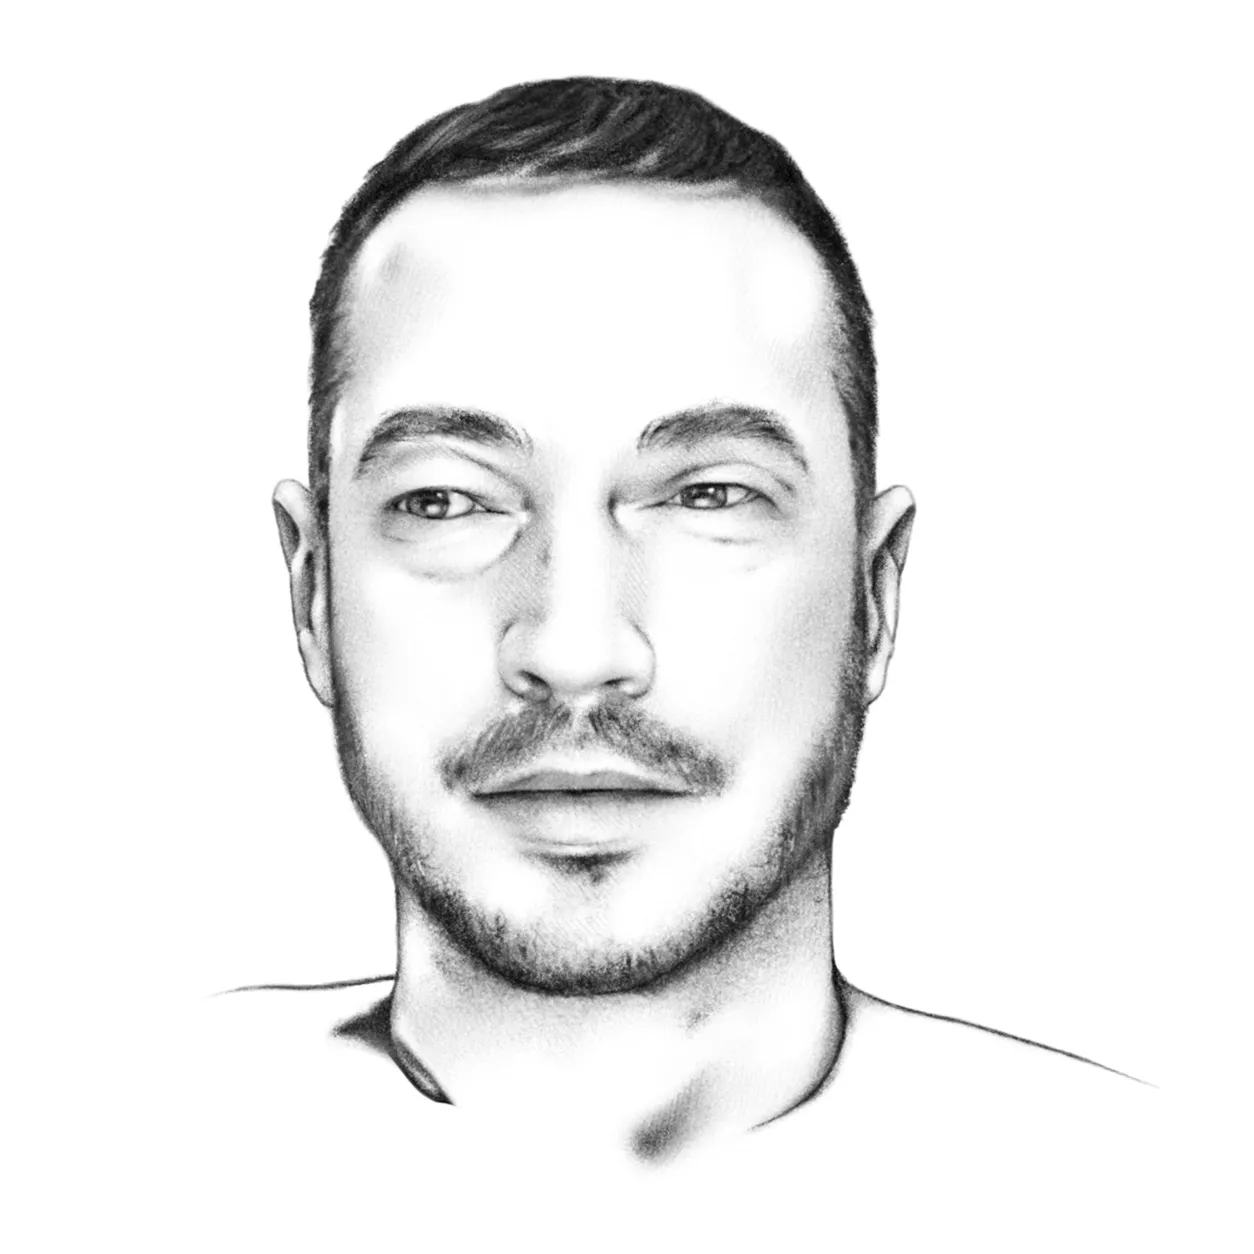
\includegraphics[width=\textwidth]{./Wired_MA_01}
	\caption{\scriptsize J. Uszkoreit}
	\label{fig:first}
\end{subfigure}
%\hfill
\begin{subfigure}{0.15\textwidth}
	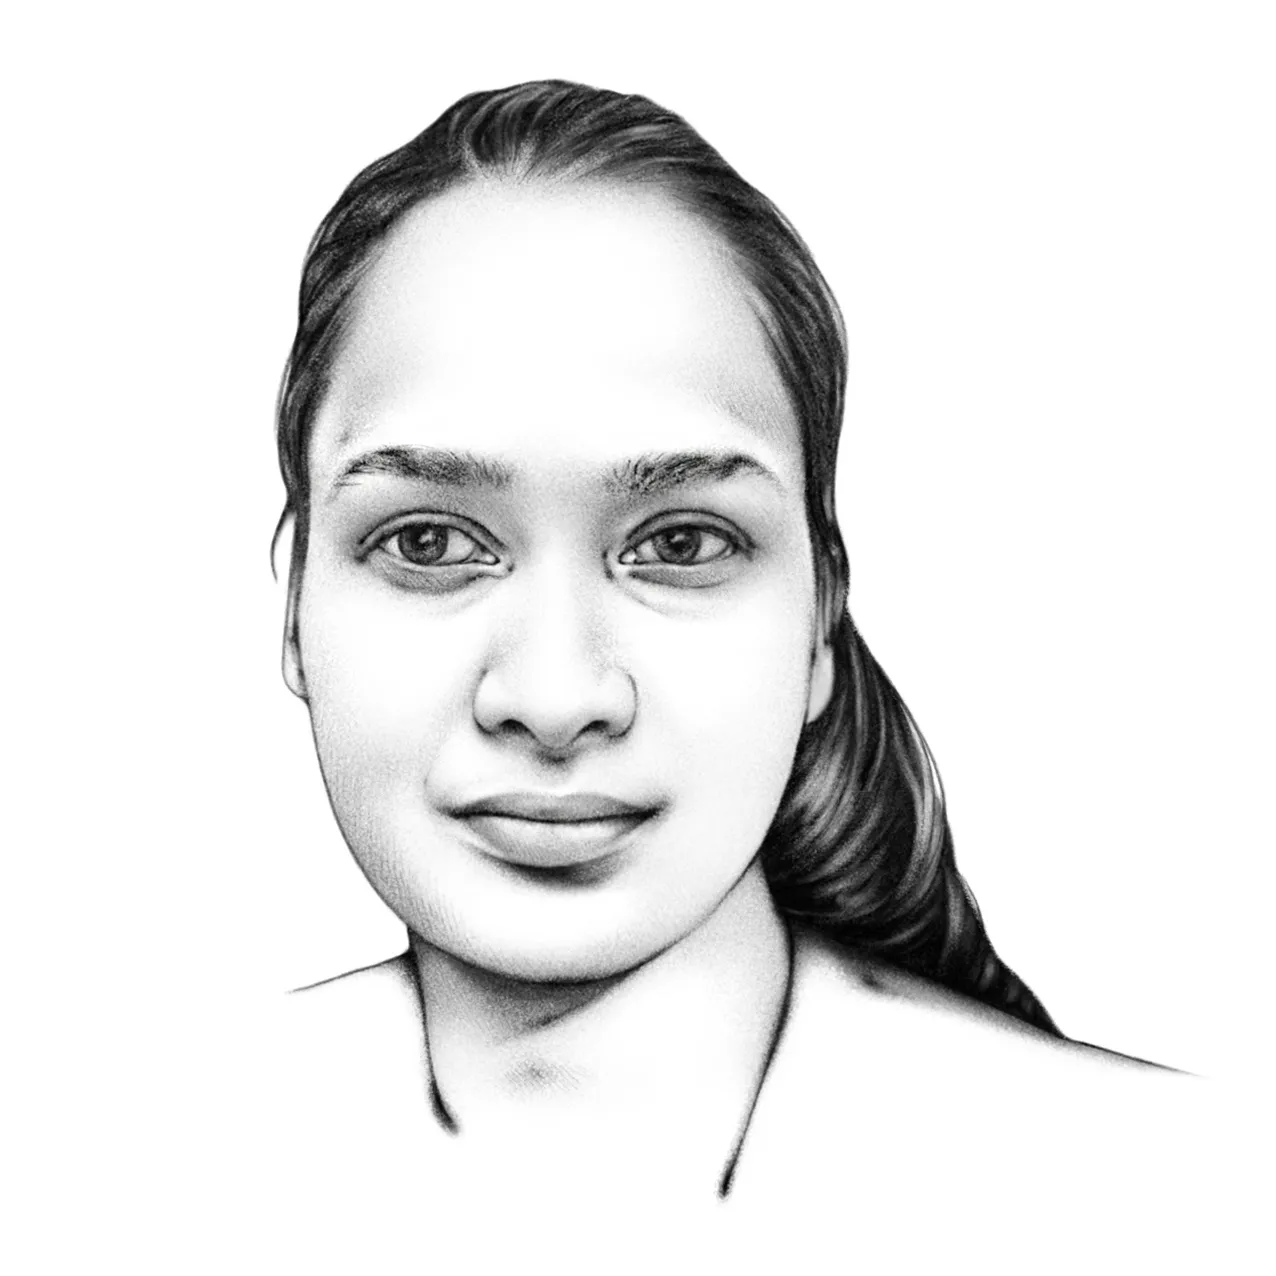
\includegraphics[width=\textwidth]{./Wired_MA_02}
	\caption{\scriptsize Niki Parmar}
	\label{fig:Niki}
\end{subfigure}
%\hfill
\begin{subfigure}{0.15\textwidth}
	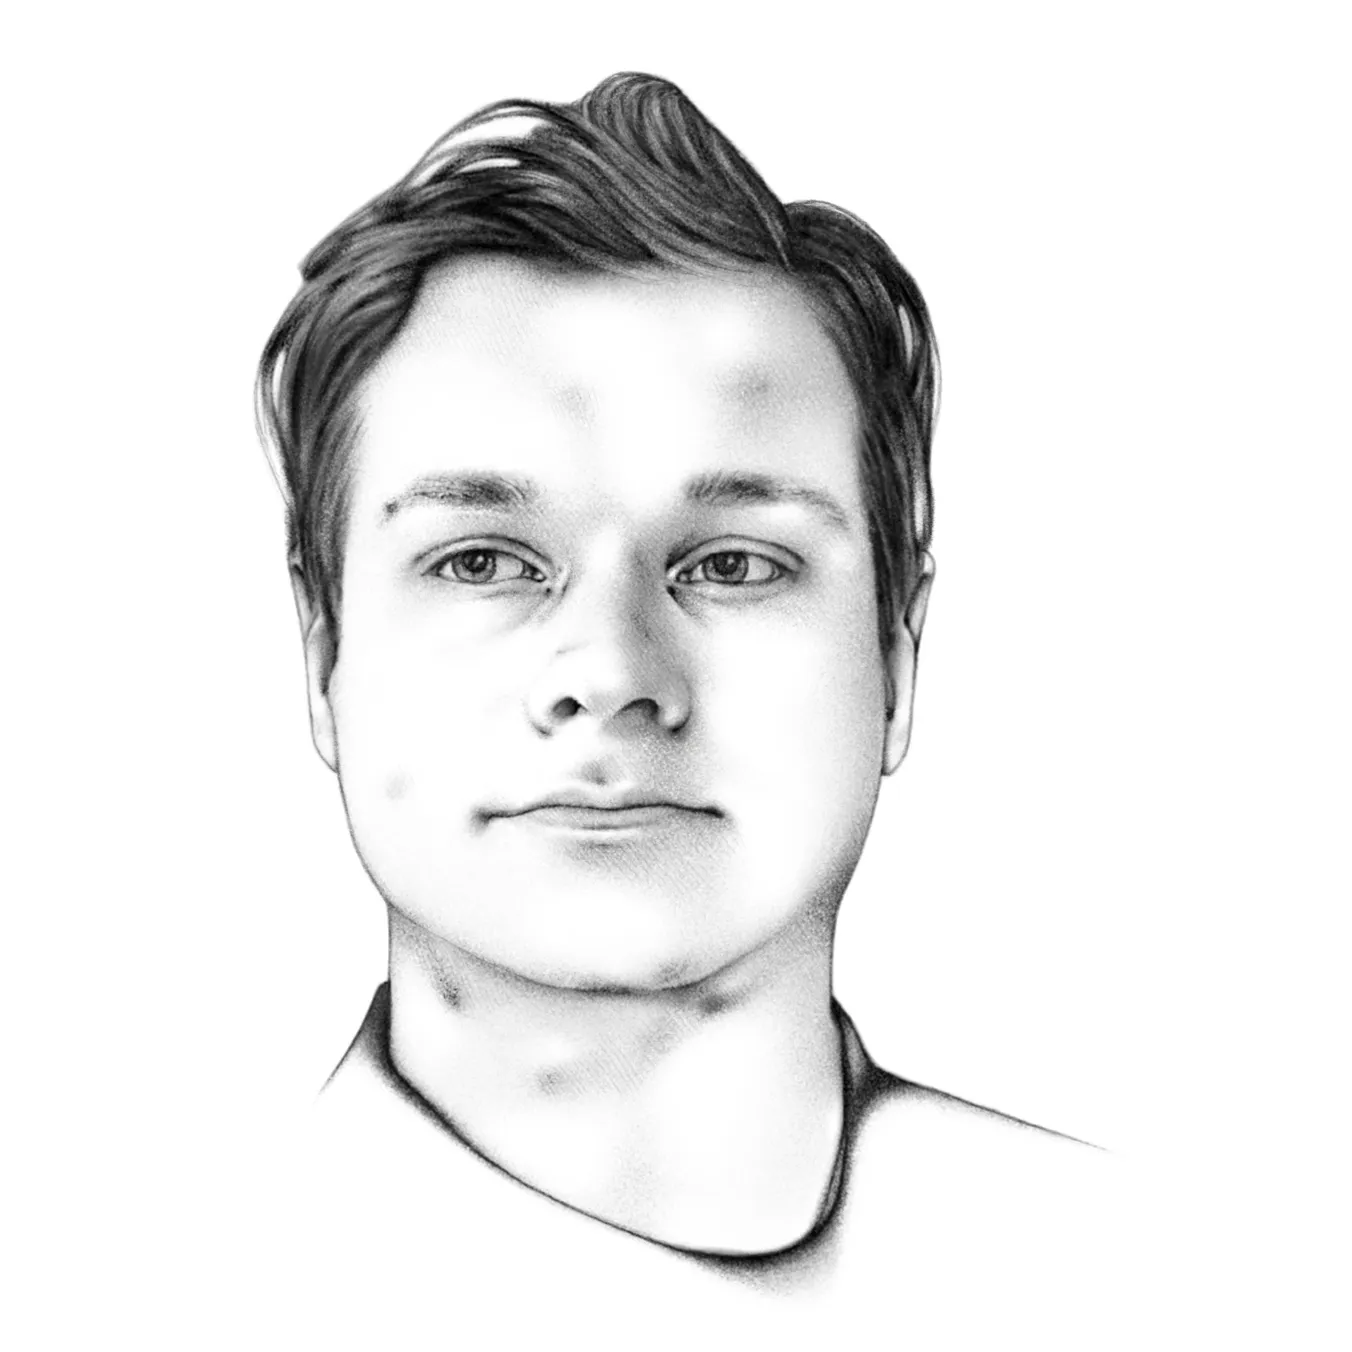
\includegraphics[width=\textwidth]{./Wired_MA_03}
	\caption{\scriptsize I. Polosukhin.}
	\label{fig:Polosukhin}
\end{subfigure}
%\hfill
\begin{subfigure}{0.15\textwidth}
	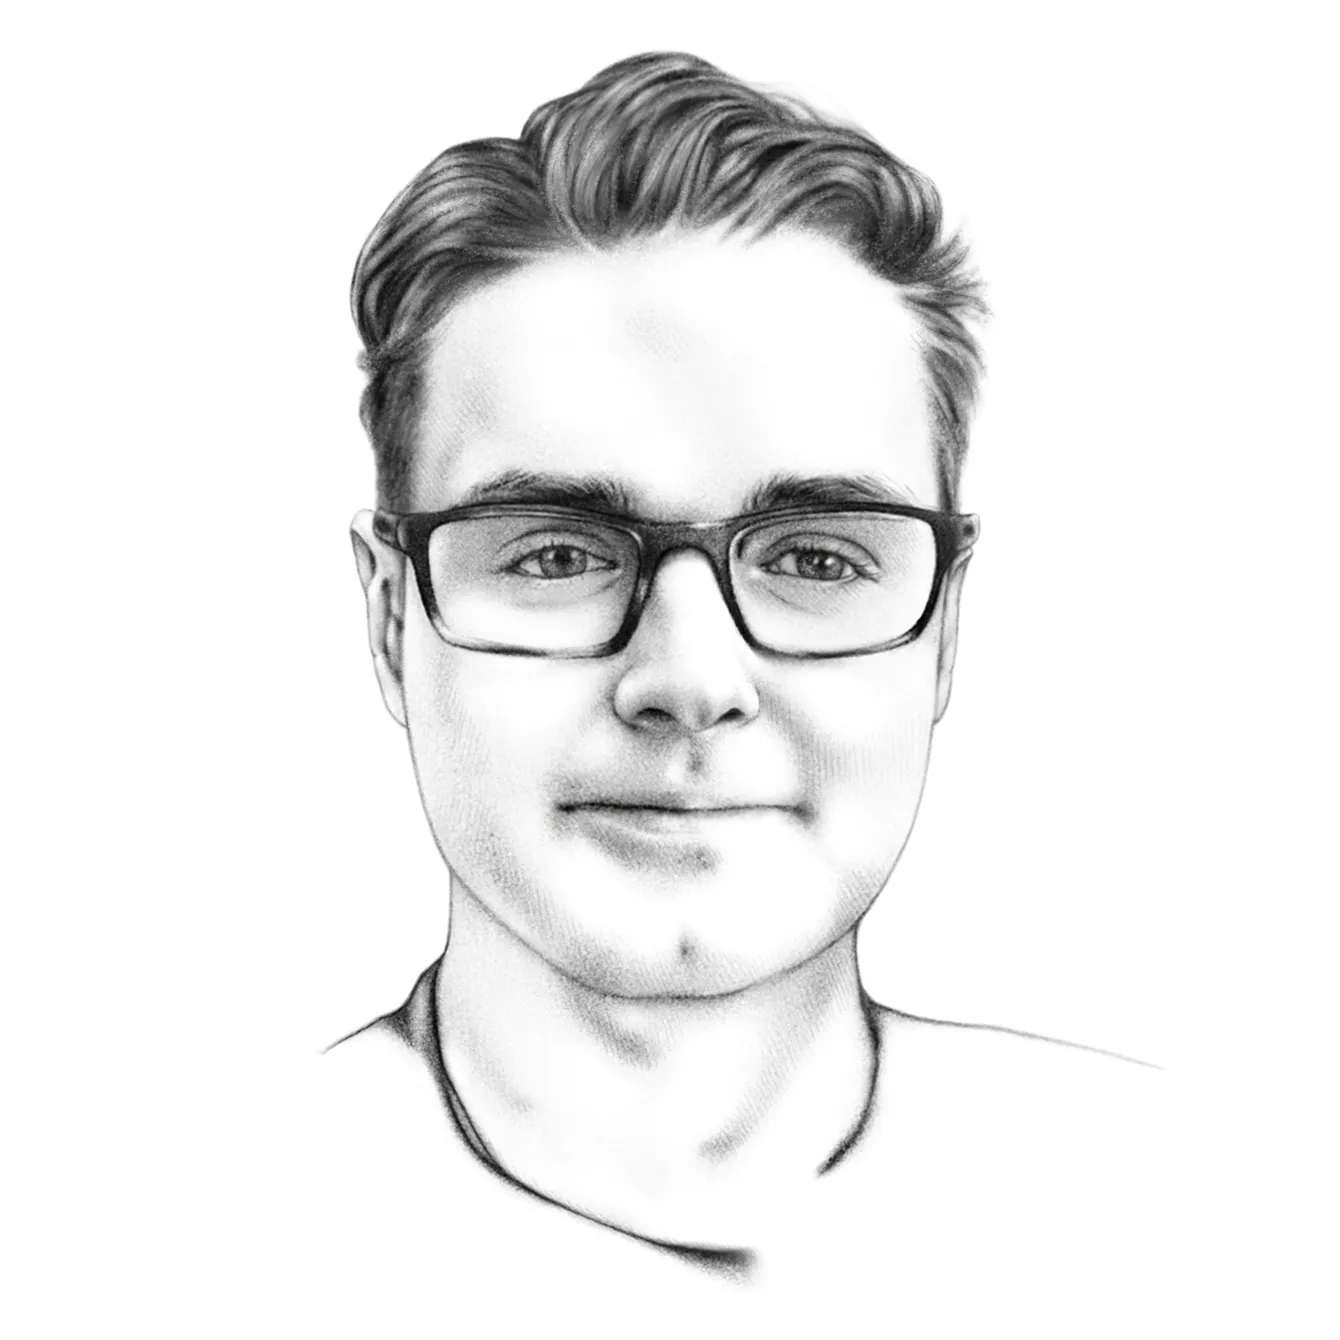
\includegraphics[width=\textwidth]{./Wired_MA_04}
	\caption{\scriptsize Llion Jones.}
	\label{fig:jones}
\end{subfigure}

\begin{subfigure}{0.15\textwidth}
	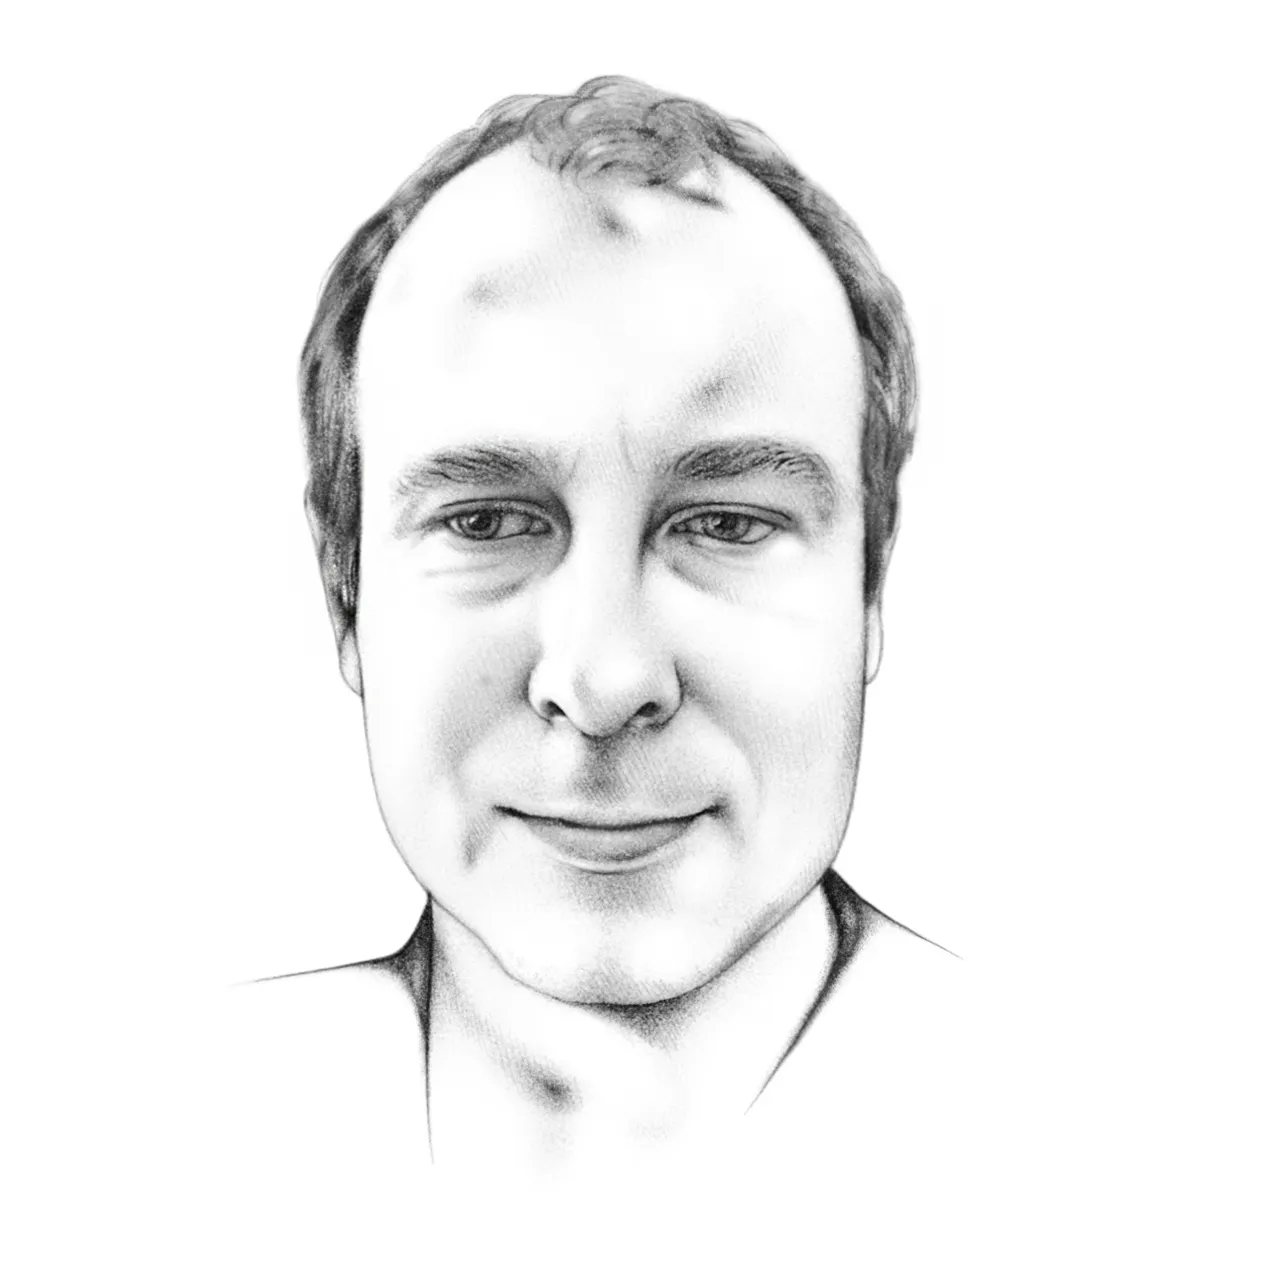
\includegraphics[width=\textwidth]{./Wired_MA_05}
	\caption{\scriptsize L. Kaizer.}
	\label{fig:lukasz}
\end{subfigure}
\begin{subfigure}{0.15\textwidth}
	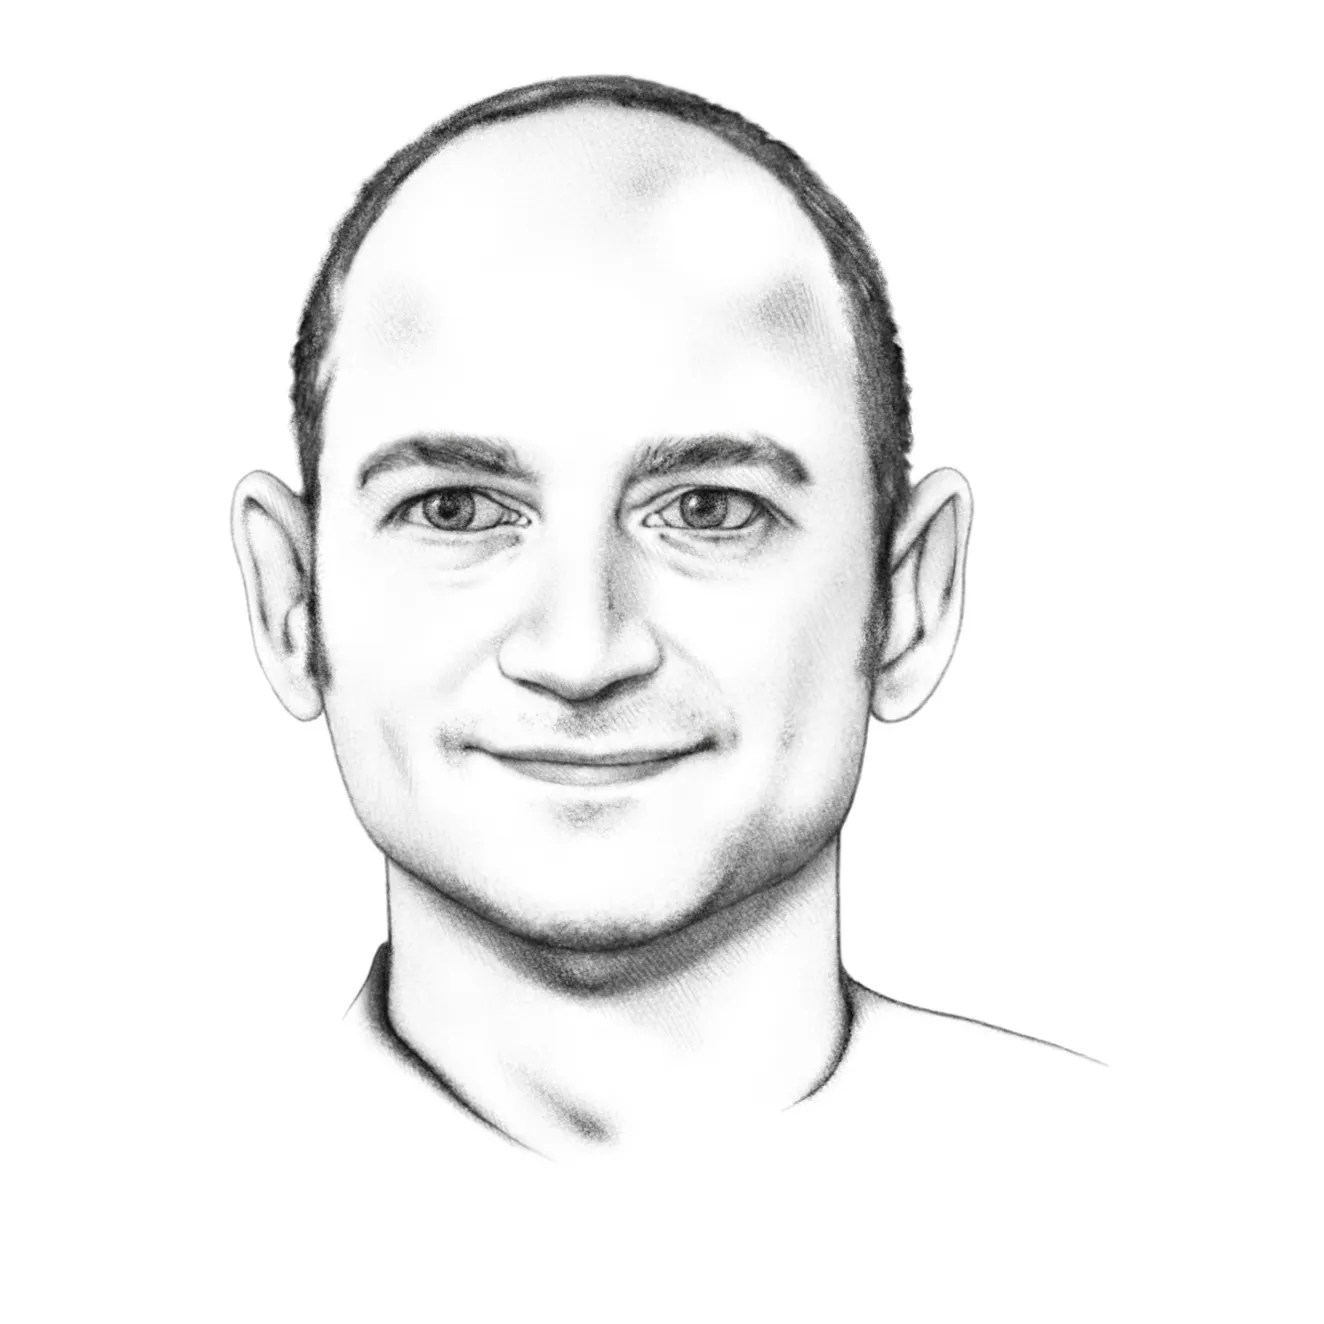
\includegraphics[width=\textwidth]{./Wired_MA_06}
	\caption{\scriptsize N. Zhazeer.}
	\label{fig:noam}
\end{subfigure}
\begin{subfigure}{0.15\textwidth}
	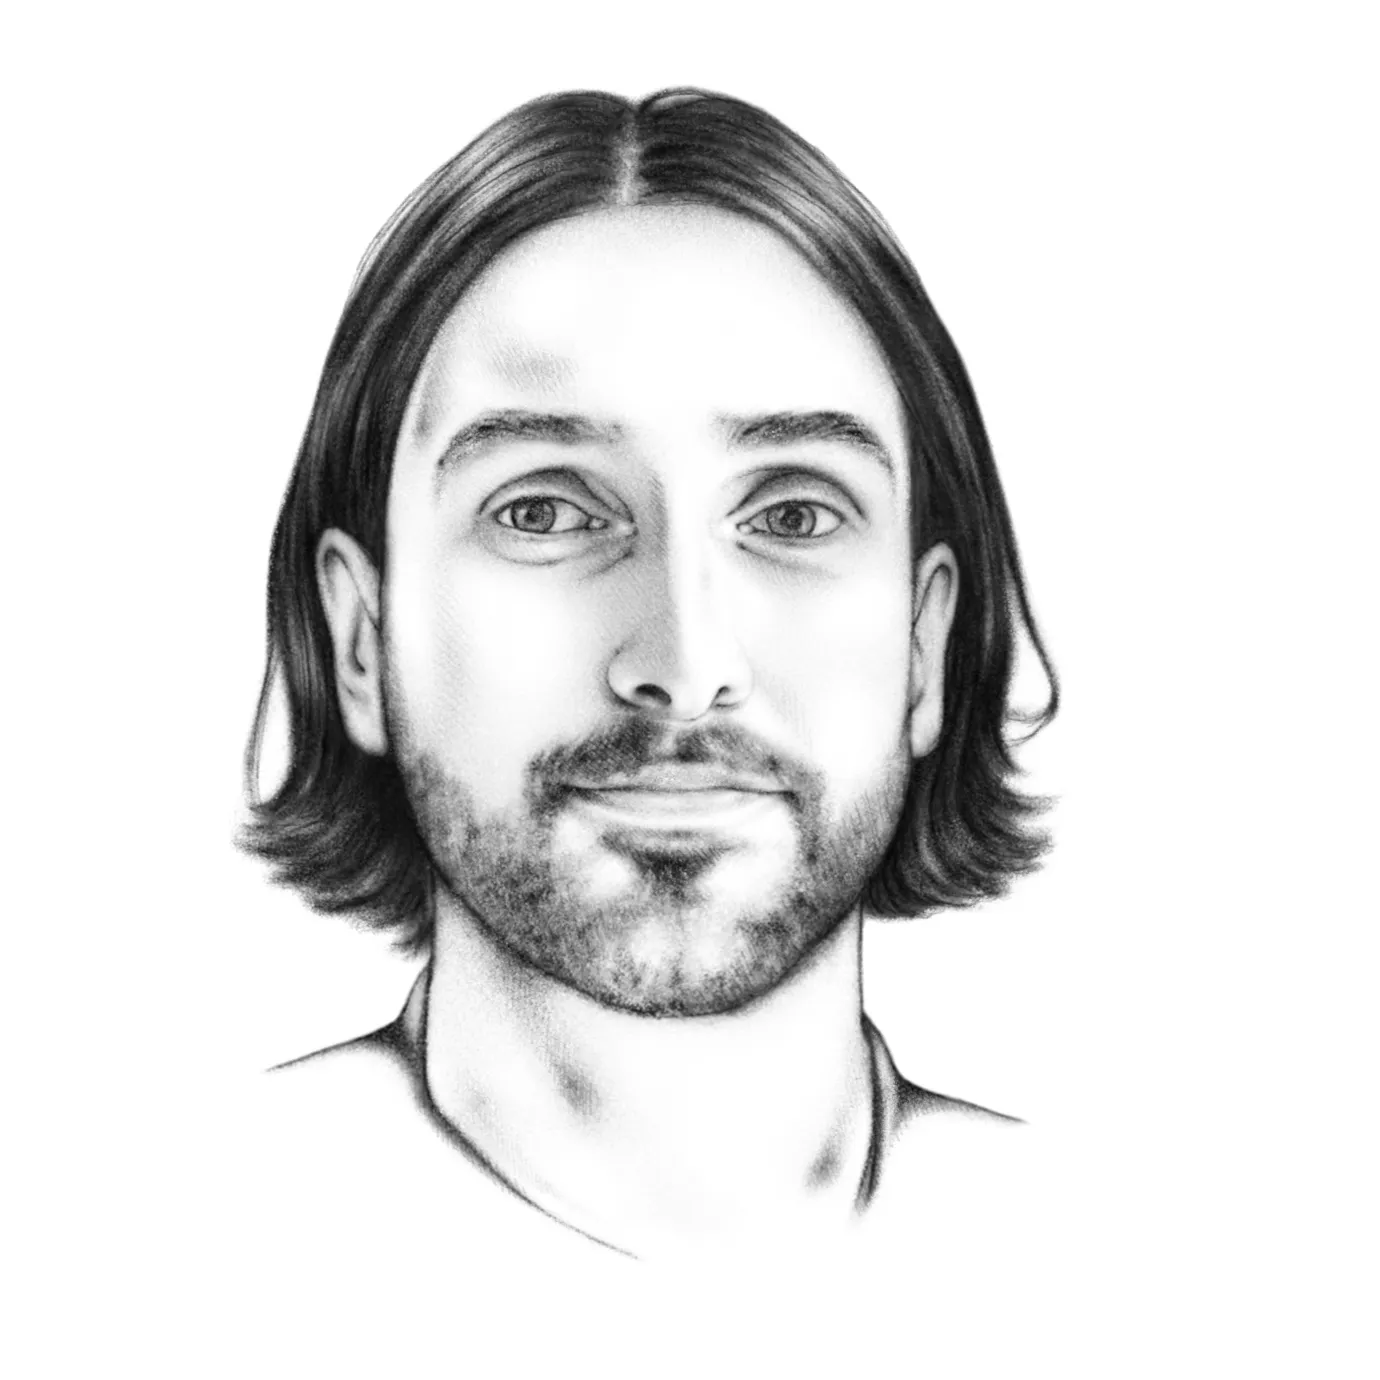
\includegraphics[width=\textwidth]{./Wired_MA_07}
	\caption{\scriptsize A.N. Gomez.}
	\label{fig:gomez}
\end{subfigure}
\begin{subfigure}{0.15\textwidth}
	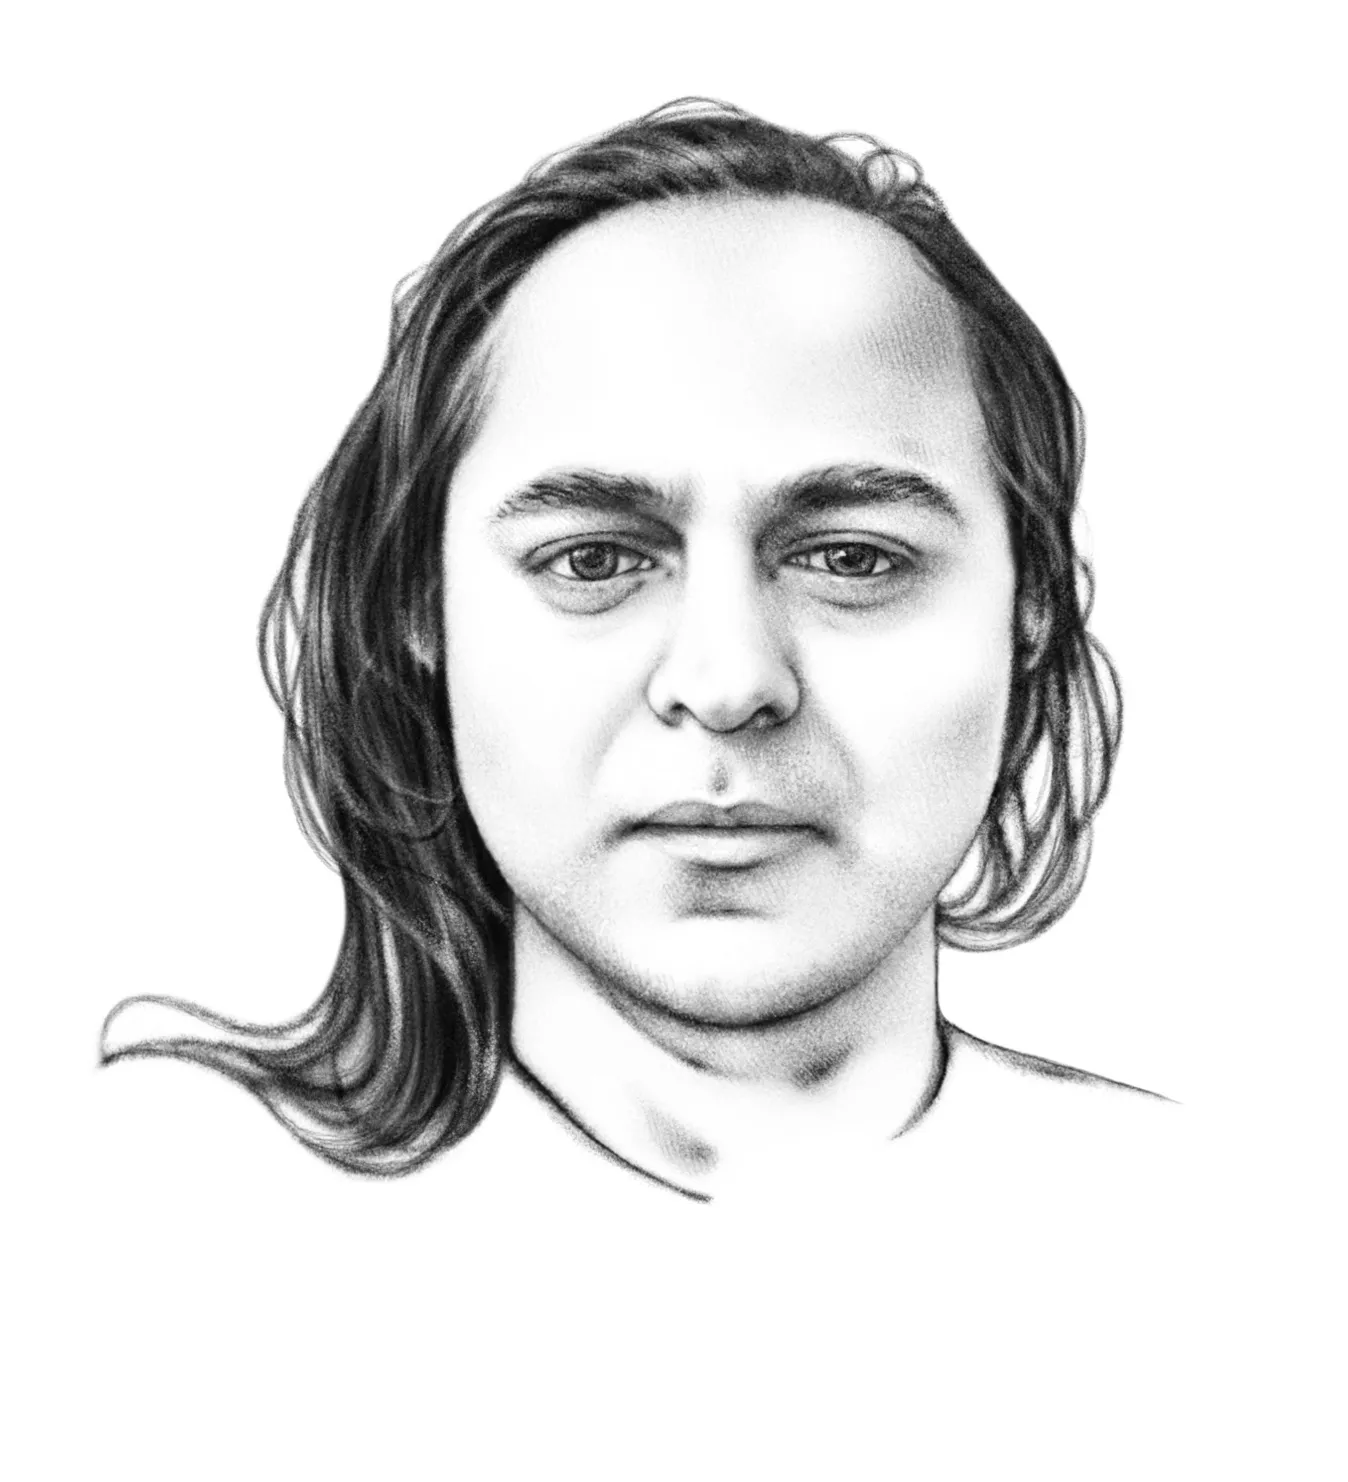
\includegraphics[width=\textwidth]{./Wired_MA_08}
	\caption{\scriptsize A. Vaswani.}
	\label{fig:vaswani}
\end{subfigure}
\end{figure}
\end{frame}



\begin{frame}
\frametitle{The transformer architecture}
\begin{figure}
	\centering
	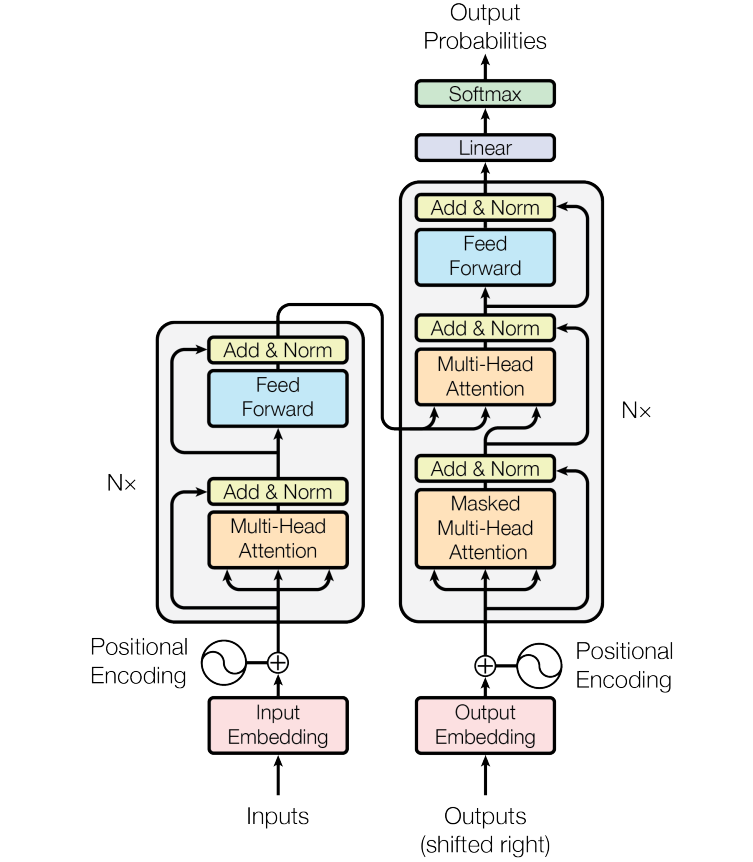
\includegraphics[height=0.85\textheight]{transformer}
	%\caption{}
	\label{fig:transformer}
\end{figure}
\end{frame}


\begin{frame}
	\frametitle{Initial explanation}
	\framesubtitle{Attention cues}
\begin{figure}
	\centering
	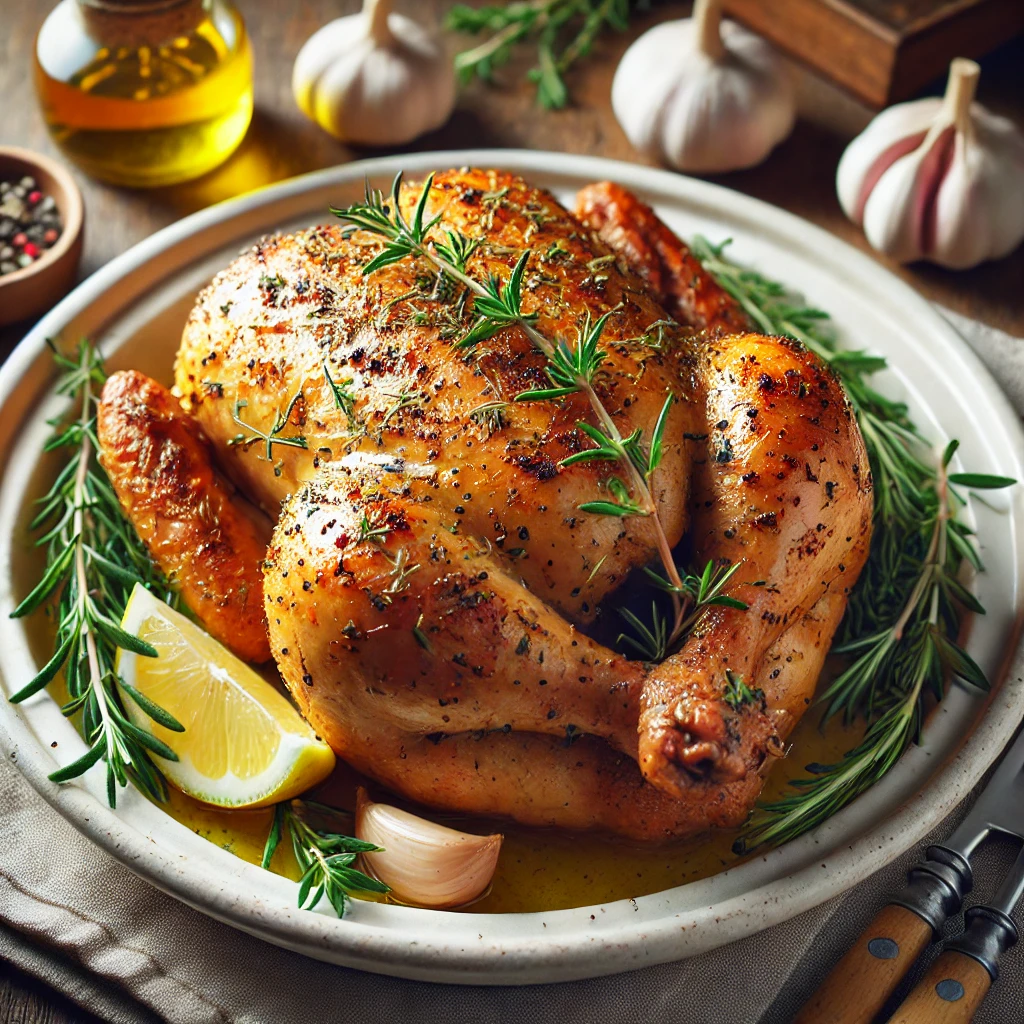
\includegraphics[width=0.3\linewidth]{pollo}
	
\includegraphics[width=0.3\linewidth]{hamaca}
	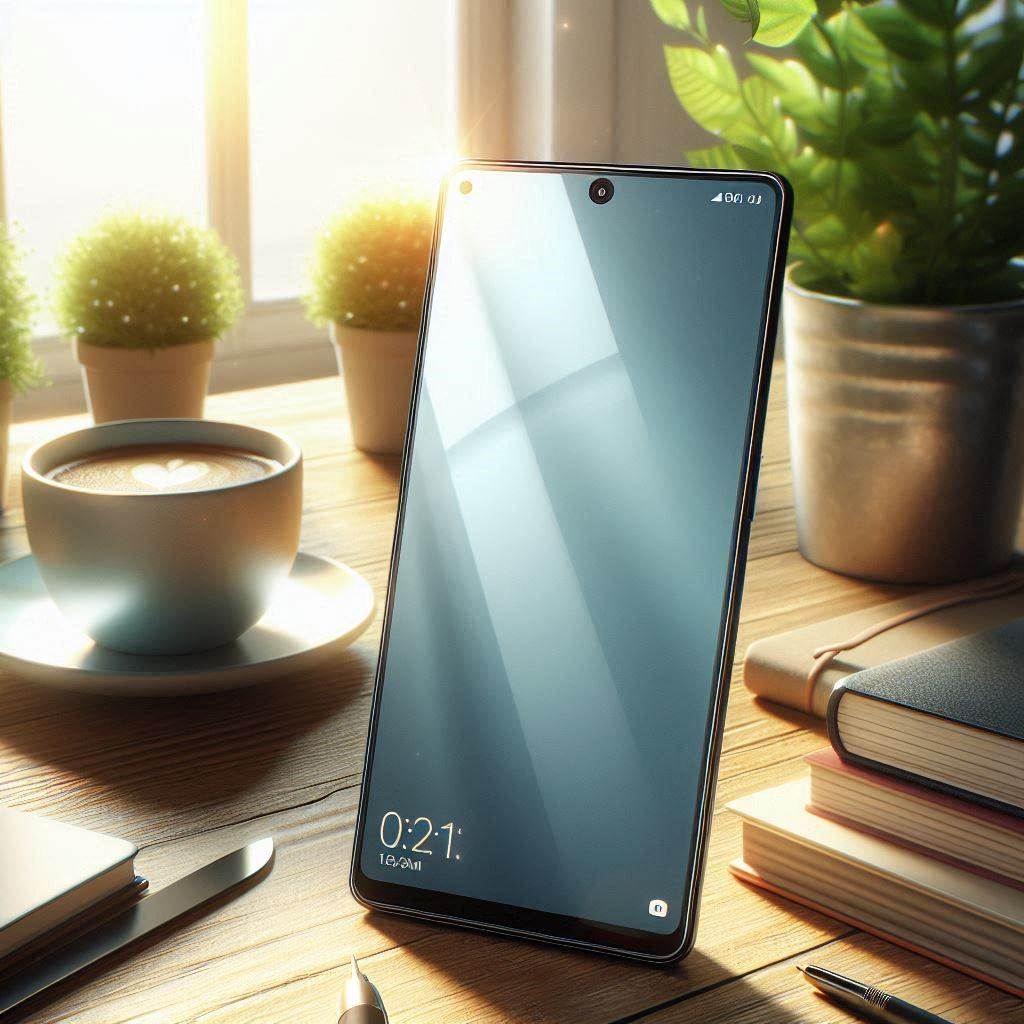
\includegraphics[width=0.3\linewidth]{tel}
	\caption{Volitional vs non-volitional cues}
	\label{fig:pollo}
\end{figure}
\end{frame}


\begin{frame}
	\frametitle{Attention}
	\begin{figure}
		\centering
		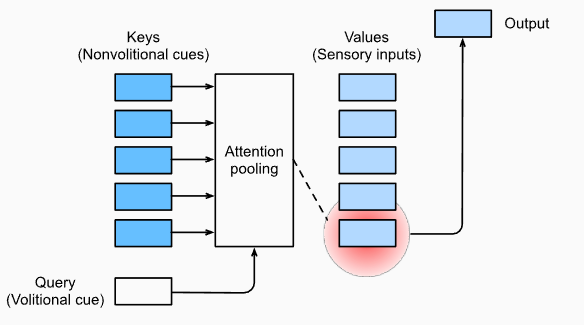
\includegraphics[height=0.7\textheight]{cues}
		\caption{Attention mechanisms bias selection over values}
		\label{fig:cues}
	\end{figure}
\end{frame}


\section{Preprocesing}


% --- Slide: Text Embeddings ---
\begin{frame}{Text Embeddings}
	\begin{columns}
		\column{0.5\textwidth}
		\begin{itemize}
			\item Allow us to manipulate word representations in meaningful ways.
			\item We can find a word similar to another, or blend two words to find one in between.
			\item This concept is key to developing \textit{attention} and subsequently \textbf{Transformers}.
		\end{itemize}
		
		\column{0.5\textwidth}
		\centering
		% Placeholder for embedding space image
		\centering
		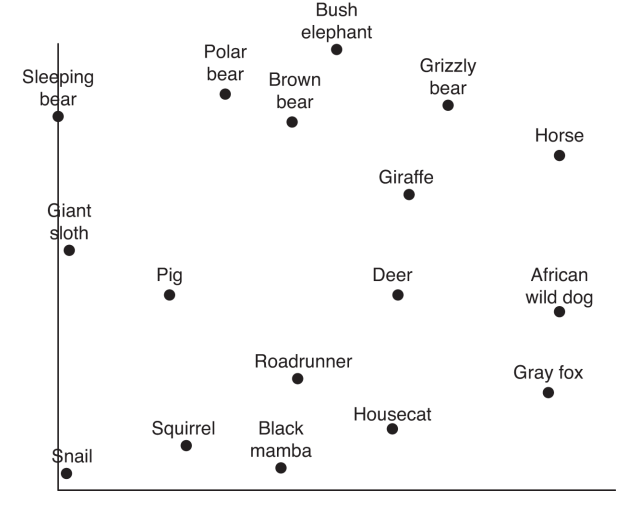
\includegraphics[width=\textwidth]{embedspace.png}
	\end{columns}
\end{frame}

% --- Slide: Embeddings arithmetic ---
\begin{frame}{Embeddings Arithmetic}
	Embeddings allow for geometric vector operations:
	
	\centering
	
	\begin{figure}
		\centering
		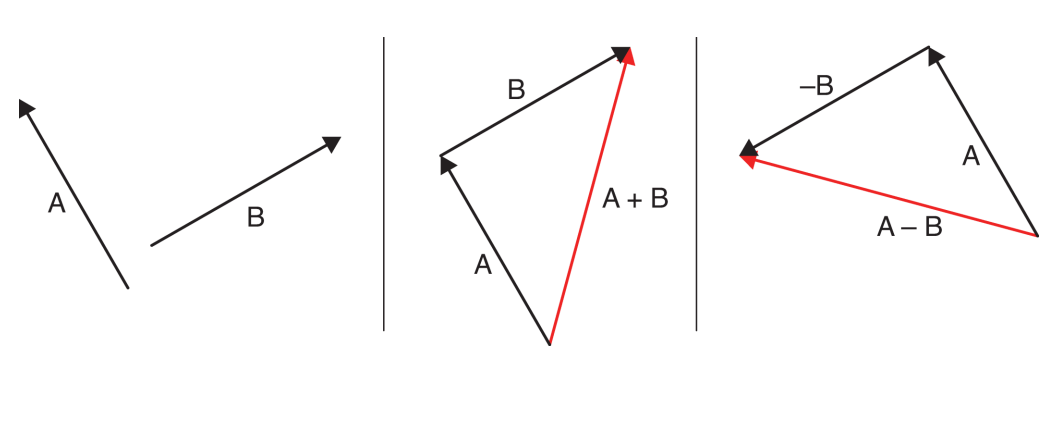
\includegraphics[width=0.7\linewidth]{enbedarith}
		\caption{Embedding arithmetics}
		\label{fig:enbedarith}
	\end{figure}
	
	\small (Visually represented as vector addition and subtraction in space).
\end{frame}

% --- Slide: Linear Structure ---
\begin{frame}{Linear Structure of Embeddings}
	Surprisingly, many semantic and syntactic relationships are (almost) linear in the word vector space.
	
	\begin{block}{Semantic Relationships}
		$$v(king) - v(man) + v(woman) \approx v(queen)$$
		\tiny
	\end{block}
	
	\begin{block}{Syntactic Relationships}
		$$v(kings) - v(king) + v(queen) \approx v(queens)$$
		\tiny
	\end{block}
	
	\vfill
	\tiny Source: Mikolov, Tomas, et al. "Efficient estimation of word representations in vector space." arXiv (2013).
\end{frame}

% --- Slide: Embedding words ---
\begin{frame}{Word Embeddings}
	\begin{itemize}
		\item A word embedding represents a word as a vector of hundreds of dimensions.
		\item Instead of assigning a single number, the algorithm assigns a list of numbers representing its coordinates in a huge space.
		\item The algorithm is called an \textit{embedder}, and the process is called \textit{embedding}.
		\item Once obtained, it is easy to incorporate them into almost any network.
		\item Instead of processing zero-dimensional tensors (single numbers), the system processes one-dimensional tensors (lists of numbers).
	\end{itemize}
\end{frame}


% --- Slide: Comparing embeddings ---
\begin{frame}{Comparing Embeddings by Similarity}
	\begin{columns}[c] % El argumento [c] alinea el contenido verticalmente en el centro
		
		% Primera Columna: Imagen
		\begin{column}{0.6\textwidth}
			\begin{figure}
				\centering
				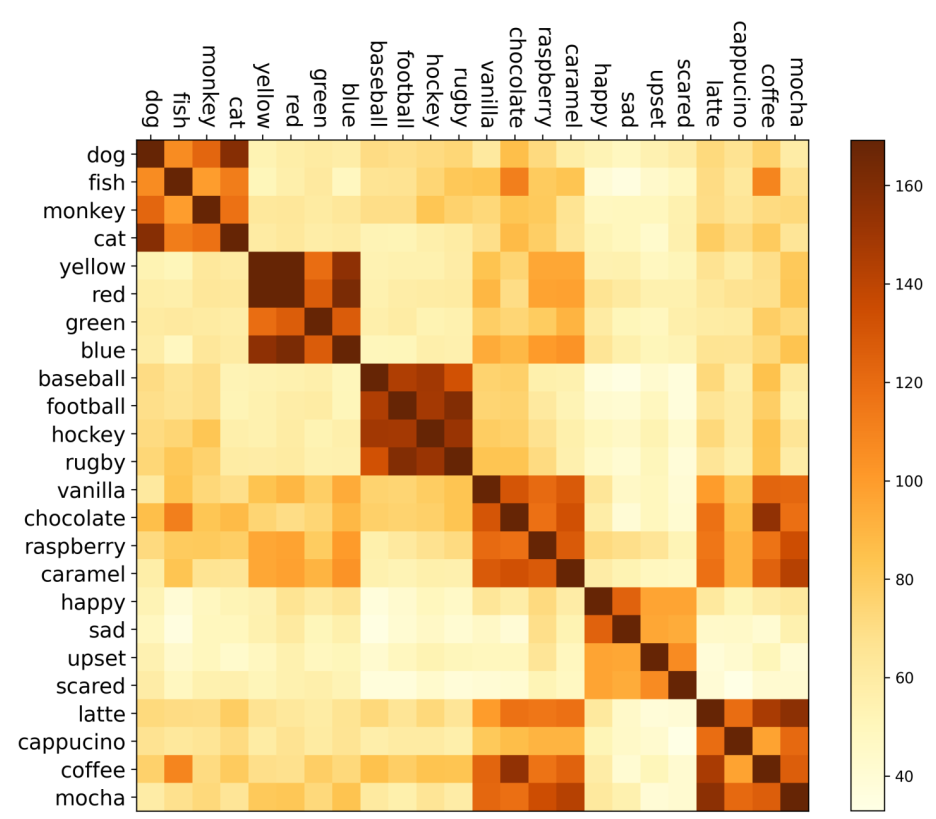
\includegraphics[width=0.8\linewidth]{embed_compar} % Ajustado a \linewidth para que se adapte bien a su columna
				\caption{Word embedding correlation}
				\label{fig:embedcompar}
			\end{figure}
		\end{column}
		
		% Segunda Columna: Texto y Lista
		\begin{column}{0.4\textwidth}
			\textbf{Famous Algorithms:}
			\begin{itemize}
				\item GloVe (2013).
				\item Word2vec (2014).
				\item fastText (2020).
			\end{itemize}
		\end{column}
		
	\end{columns}
\end{frame}


% --- Slide: Embed sentences ---
\begin{frame}{Sentence Embeddings\footnote{Cer, Daniel, et al. "Universal Sentence Encoder." arXiv (2018).}}
	\begin{figure}
		\centering
		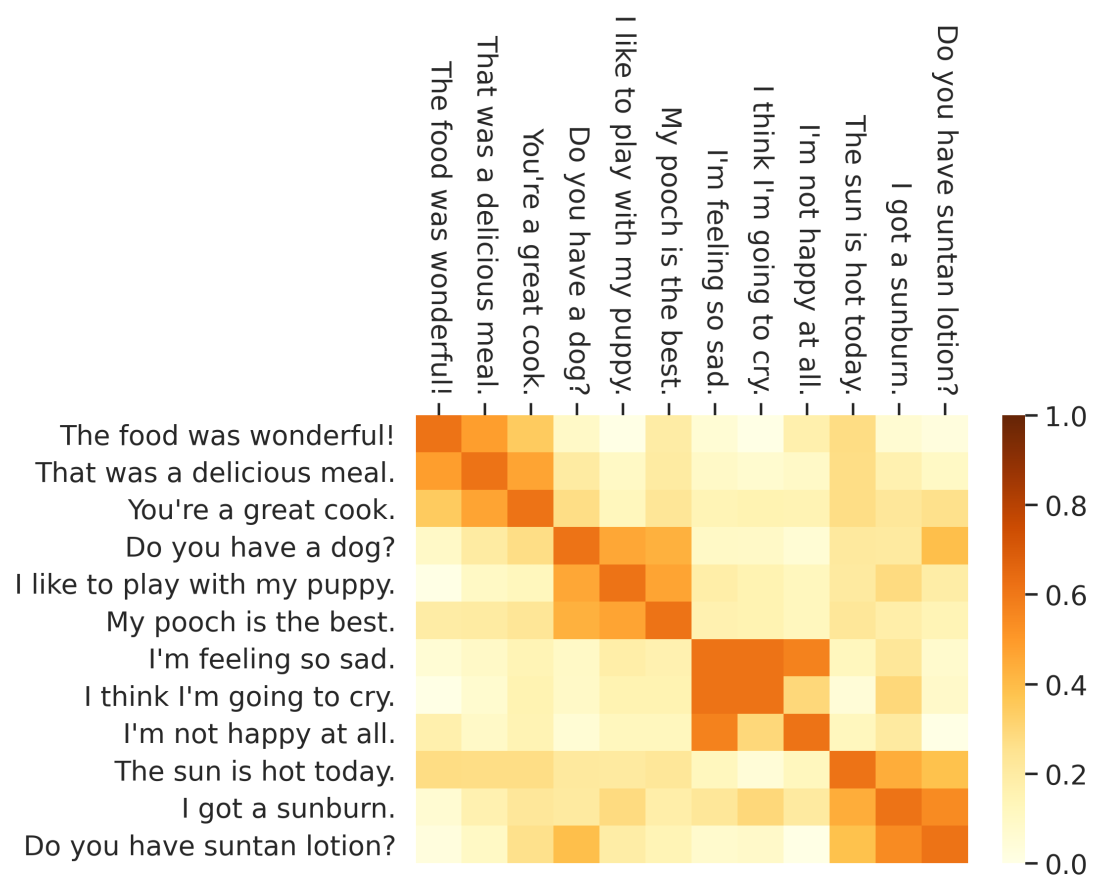
\includegraphics[width=0.45\linewidth]{embedsent}
		\caption{Correlation of embedded sentences}
		\label{fig:embedsent}
	\end{figure}
\end{frame}


% --- Slide: Problem with Word embeddings ---
\begin{frame}{The Problem with Static Word Embeddings}
	Many languages have words with different meanings that are written the same way (homonyms).
	
	\textbf{The case of the word "train":}
	\begin{itemize}
		\item Noun: "I rode on a \textbf{train}".
		\item Verb: "I like to \textbf{train} dogs".
	\end{itemize}
	
	\begin{alertblock}{Limitation}
		If we assign a single static embedding to "train", we mix two entirely different ideas. We need to distinguish meanings based on context.
	\end{alertblock}
	
	\textit{This leads us to the need for contextualized embeddings (like ELMo and Transformers).}
\end{frame}


\begin{frame}
	\frametitle{Positional encoding}
	For a given position $\text{pos}$ and a dimension index $i$ within the embedding vector:$$PE_{(\text{pos}, 2i)} = \sin\left(\frac{\text{pos}}{10000^{\frac{2i}{d_{\text{model}}}}}\right)$$$$PE_{(\text{pos}, 2i+1)} = \cos\left(\frac{\text{pos}}{10000^{\frac{2i}{d_{\text{model}}}}}\right)$$
\end{frame}


\begin{frame}
	\frametitle{Positional encoding}
	\begin{figure}
		\centering
		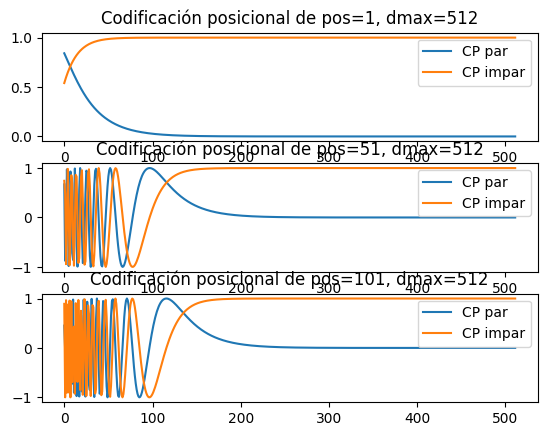
\includegraphics[height=0.7\textheight]{pe_example}
		%\caption{}
		\label{fig:peexample}
	\end{figure}
\end{frame}


\section{Attention mechanism}


\begin{frame}
	\frametitle{Previous attention}
	Attention function is used for correlating, which allows the similarity computations between samples. Steps
	\begin{enumerate}
		\item Computing the similarity between $Q$ and $K$:
		\begin{equation}
			f(Q,K_i), i = 1,2 \dots m
		\end{equation}
		\item Normalizing the obtained similarity:
		\begin{equation}
			\alpha_i = \frac{f(Q,K_i)}{\sum_{j=1}^{m} f(Q,K_i)}, i = 1,2 \dots m 
		\end{equation}
		\item Computing the weighted sum of V with the weight $\alpha_i$:
		\begin{equation}
			Attention(Q, K, V ) = \sum_{i=1}^{m} \alpha_i V_i
		\end{equation}
	\end{enumerate}
\end{frame}

\begin{frame}
	\frametitle{Attention mechanism (Vaswani et al. 2017)}
\begin{figure}
	\centering
	\includegraphics[height=0.75\textheight]{"scaled dot product"}
	\caption{Scaled dot-product attention}
	\label{fig:scaled-dot-product}
\end{figure}
\end{frame}



% Slide 1: Concept and Intuition
\begin{frame}{From Input to Attention Spaces}
	The input matrix $X$ (comprising token embeddings and positional encodings) is linearly projected into three separate vector spaces:
	
	\vspace{0.4cm}
	\begin{columns}[T]
		\begin{column}{0.31\textwidth}
			\begin{block}{\centering \rule{0pt}{2ex} Query ($Q$)}
				\small
				\textbf{What am I looking for?} \\
				Represents the current token's focus or "question" directed at the rest of the sequence.
			\end{block}
		\end{column}
		
		\begin{column}{0.31\textwidth}
			\begin{block}{\centering \rule{0pt}{2ex} Key ($K$)}
				\small
				\textbf{What do I offer?} \\
				Represents the relevance label of a token. It is used to match against incoming Queries.
			\end{block}
		\end{column}
		
		\begin{column}{0.31\textwidth}
			\begin{block}{\centering \rule{0pt}{2ex} Value ($V$)}
				\small
				\textbf{What do I contain?} \\
				Holds the actual semantic content that will be extracted if a strong match occurs.
			\end{block}
		\end{column}
	\end{columns}
\end{frame}

% Slide 2: Mathematical Formulation
\begin{frame}{Mathematical Formulation}
	Each matrix is generated by multiplying the input matrix $X$ by its respective learnable weight matrix:
	
	\begin{equation}
			Q = X \cdot W^Q
	\end{equation}

	\begin{equation}
			K = X \cdot W^K
\end{equation}

	\begin{equation}
			V = X \cdot W^V
\end{equation}	
	
The projection weight matrices $W^Q, W^K,$ and $W^V$ are randomly initialized and optimized end-to-end via backpropagation during training.
\end{frame}


% Slide 3: Dimensionality Analysis
\begin{frame}{Dimensionality Analysis (Base Model: \textit{Vaswani et al.})}
	In the original Transformer architecture, dimensions are scaled down to enable efficient parallel processing via multiple attention heads (\textit{Multi-Head Attention}):
	
	\vspace{0.4cm}
	\centering
	\begin{tabular}{lccc}
		%\toprule
		\textbf{Element} & \textbf{Matrix} & \textbf{Algebraic Dimension} & \textbf{Actual Size ($n = $ tokens)} \\
		%\midrule
		Input Sequence & $X$ & $n \times d_{\text{model}}$ & $n \times 512$ \\
		%\addlinespace
		Projection Weights & $W^Q, W^K, W^V$ & $d_{\text{model}} \times d_k$ & $512 \times 64$ \\
		%\addlinespace
		%\midrule
		\textbf{Projected Output} & \textbf{$Q, K, V$} & $\mathbf{n \times d_k}$ & $\mathbf{n \times 64}$ \\
		%\bottomrule
	\end{tabular}
	
	\vspace{0.4cm}
	\small
	\textcolor{gray}{By projecting from dimension $512$ down to $64$, each attention head can independently specialize in a distinct representation subspace without increasing the overall computational cost.}
\end{frame}


\begin{frame}
	\frametitle{Attention mechanism (Vaswani et al. 2017)}
Given a Query ($K$), Keys ($K$), and values ($V$), the attention is defined as: 
	\begin{equation}
\text{Attention}(Q, K, V) =  \text{softmax}\left(\frac{QK^T}{\sqrt{d_k}}\right) V 
	\end{equation}	where $d_k$ is the dimension of que queries and keys.
\end{frame}


\begin{frame}
	\frametitle{Multi-head attention}
\begin{figure}
	\centering
	\includegraphics[height=0.7\textheight]{"multihead attention"}
	\caption{Multi-Head Attention consists of several
		attention layers running in parallel}
	\label{fig:multihead-attention}
\end{figure}
\end{frame}


\begin{frame}
	\frametitle{Multi-head attention}
	\begin{equation}
\text{MultiHeadAttention}(Q, K, V) = \text{Concat}(\text{head}_1, \text{head}_2, \ldots, \text{head}_h) W^O
	\end{equation} where

\begin{equation}
\quad \text{head}_i = \text{Attention}(QW_{i}^Q, KW_{i}^K, VW_{i}^V)
\end{equation}
\end{frame}


%
%\begin{frame}
%	\frametitle{title}
%\end{frame}


\frame{
	\frametitle{Lets think about it}
	\framesubtitle{The I.A. revolution:}
	\begin{columns}
		\column{0.5\linewidth}
		What we though the I.A. will be: \\
		\vspace{0.7cm}
		
\includegraphics[width=1.0\textwidth]{Gemini_Generated_Image_xfouuzxfouuzxfou.png}
		\pause
		\column{0.5\linewidth}
		What it is really doing: \\
		\vspace{0.7cm}
		
\includegraphics[width=1.0\textwidth]{hq720.jpg}
		
	\end{columns}
}


\begin{frame}
	\frametitle{References}
	\begin{itemize}
		\item Wired Magazine, 8 Google Employees Invented Modern AI, https://www.wired.com/
		\item Goodfellow, Ian, Yoshua Bengio, and Aaron Courville. Deep learning. MIT press, 2016.
		\item Zhang, Aston, et al. "Dive into deep learning." arXiv preprint arXiv:2106.11342 (2021).
	\end{itemize}
\end{frame}

\end{document}